\documentclass[11pt]{article}
\usepackage[a4paper,margin=28mm]{geometry}
\usepackage[T1]{fontenc}
\usepackage{lmodern,amsmath,amssymb,amsthm,mathtools,microtype}
\usepackage[numbers,sort&compress]{natbib}
\usepackage{tikz}
\usetikzlibrary{arrows.meta,positioning}
\usepackage[hyphens]{url}
\usepackage{hyperref}
\newcommand{\doi}[1]{\href{https://doi.org/#1}{\nolinkurl{doi:#1}}}
\input{glyphtounicode}
\pdfglyphtounicode{angbracketleftBigg}{27E8}
\pdfglyphtounicode{angbracketleftbig}{27E8}
\pdfglyphtounicode{angbracketrightBigg}{27E9}
\pdfglyphtounicode{angbracketrightbig}{27E9}
\pdfglyphtounicode{arrowhookleft}{02D3}
\pdfglyphtounicode{axisshort}{002D}
\pdfglyphtounicode{arrowaxisright}{2192}
\pdfglyphtounicode{circleplusdisplay}{2A01}
\pdfglyphtounicode{braceex}{23AA}
\pdfglyphtounicode{braceleftbigg}{007B}
\pdfglyphtounicode{braceleftbt}{23A9}
\pdfglyphtounicode{braceleftmid}{23A8}
\pdfglyphtounicode{bracelefttp}{23A7}
\pdfglyphtounicode{bracerightbigg}{007D}
\pdfglyphtounicode{bracketleftbig}{005B}
\pdfglyphtounicode{bracketleftbigg}{005B}
\pdfglyphtounicode{bracketleftbt}{23A3}
\pdfglyphtounicode{bracketlefttp}{23A1}
\pdfglyphtounicode{bracketrightbig}{005D}
\pdfglyphtounicode{bracketrightbigg}{005D}
\pdfglyphtounicode{bracketrightbt}{23A6}
\pdfglyphtounicode{bracketrighttp}{23A4}
\pdfglyphtounicode{hatwide}{0302}
\pdfglyphtounicode{hatwider}{0302}
\pdfglyphtounicode{hatwidest}{0302}
\pdfglyphtounicode{integraldisplay}{222B}
\pdfglyphtounicode{integraltext}{222B}
\pdfglyphtounicode{intersectiondisplay}{22C2}
\pdfglyphtounicode{intersectiontext}{22C2}
\pdfglyphtounicode{mapsto}{007C}
\pdfglyphtounicode{parenleftBig}{0028}
\pdfglyphtounicode{parenleftBigg}{0028}
\pdfglyphtounicode{parenleftbig}{0028}
\pdfglyphtounicode{parenleftbigg}{0028}
\pdfglyphtounicode{parenleftbt}{239D}
\pdfglyphtounicode{parenlefttp}{239B}
\pdfglyphtounicode{parenrightBig}{0029}
\pdfglyphtounicode{parenrightBigg}{0029}
\pdfglyphtounicode{parenrightbig}{0029}
\pdfglyphtounicode{parenrightbigg}{0029}
\pdfglyphtounicode{parenrightbt}{23A0}
\pdfglyphtounicode{parenrighttp}{239E}
\pdfglyphtounicode{productdisplay}{220F}
\pdfglyphtounicode{producttext}{220F}
\pdfglyphtounicode{radicalbig}{221A}
\pdfglyphtounicode{radicalbigg}{221A}
\pdfglyphtounicode{radicalBigg}{221A}
\pdfglyphtounicode{floorleftbigg}{230A}
\pdfglyphtounicode{floorrightbigg}{230B}
\pdfglyphtounicode{ceilingleftBig}{2308}
\pdfglyphtounicode{ceilingrightBig}{2309}
\pdfglyphtounicode{summationdisplay}{2211}
\pdfglyphtounicode{summationtext}{2211}
\pdfglyphtounicode{uniontext}{22C3}
\pdfglyphtounicode{vextenddouble}{2225}
\pdfglyphtounicode{vextendsingle}{007C}
\pdfglyphtounicode{tildewide}{0303}
\pdfglyphtounicode{tildewider}{0303}
\pdfglyphtounicode{bracketleftBigg}{005B}
\pdfglyphtounicode{bracketrightBigg}{005D}
\pdfglyphtounicode{braceleftBigg}{007B}
\pdfglyphtounicode{bracerightBigg}{007D}
\pdfglyphtounicode{braceleftBig}{007B}
\pdfglyphtounicode{bracerightBig}{007D}
\pdfglyphtounicode{coproductdisplay}{2210}
\pdfglyphtounicode{bracketleftBig}{005B}
\pdfglyphtounicode{bracketrightBig}{005D}
\pdfglyphtounicode{radicalBig}{221A}
\pdfglyphtounicode{uniondisplay}{22C3}
\pdfglyphtounicode{logicalandtext}{22C0}
\pdfglyphtounicode{logicalanddisplay}{22C0}
\pdfglyphtounicode{circlemultiplytext}{2A02}
\pdfglyphtounicode{circlemultiplydisplay}{2A02}
\pdfglyphtounicode{braceleftbig}{007B}
\pdfglyphtounicode{bracerightbig}{007D}
\pdfglyphtounicode{bracerighttp}{23AB}
\pdfglyphtounicode{bracerightmid}{23AC}
\pdfglyphtounicode{bracerightbt}{23AD}
\pdfgentounicode=1

\pdfinfoomitdate=1
\pdftrailerid{}
\pdfsuppressptexinfo=15
\hypersetup{colorlinks=true,linkcolor=blue,citecolor=blue,urlcolor=blue,
 pdftitle={Invariant-projection counterexamples for every irrational rotation},
 pdfauthor={OpenAI}}
\newcommand{\R}{\mathbb R}
\newcommand{\Z}{\mathbb Z}
\newcommand{\N}{\mathbb N}
\newcommand{\C}{\mathbb C}
\newcommand{\T}{\mathbb T}
\newcommand{\ind}{\mathbf 1}
\DeclareMathOperator{\diag}{diag}
\DeclareMathOperator{\ran}{ran}
\newtheorem{theorem}{Theorem}[section]
\newtheorem{lemma}[theorem]{Lemma}
\newtheorem{proposition}[theorem]{Proposition}
\newtheorem{corollary}[theorem]{Corollary}
\theoremstyle{definition}
\newtheorem{definition}[theorem]{Definition}
\theoremstyle{remark}
\newtheorem{remark}[theorem]{Remark}
\numberwithin{equation}{section}
\setlength{\emergencystretch}{2em}
\title{Invariant-projection counterexamples\\for every irrational rotation}
\author{OpenAI}
\date{September 27, 2026}
\begin{document}
\maketitle
\begin{abstract}
For every irrational angle, we construct a continuous nonnegative circle
weight with exactly one zero and logarithmic integral $-\infty$ whose
weighted rotation has no nontrivial invariant projection in the associated
hyperfinite type $\mathrm{II}_1$ factor. This answers negatively the question
of Zhu, Fang, and Shi, with the angle prescribed in advance. The resulting
operator is nonzero and norm-quasinilpotent.
\end{abstract}
\section{Introduction}\label{sec:introduction}

Let $\theta\in(0,1)$ be irrational.  In the tracial representation let
$R_\theta$ be the von Neumann algebra generated by unitaries $U,V$ with
\[
 VU=e^{2\pi i\theta}UV,\qquad
 \tau(U^mV^n)=0\quad((m,n)\in\Z^2\setminus\{(0,0)\}),\qquad\tau(1)=1.
\]
This is the hyperfinite factor of type $\mathrm{II}_1$; the concrete
representation used below is the group-measure-space representation of
irrational rotation.  For a continuous function $f$ on the unit circle
$\T$, write $T_f=Uf(V)$.  A closed invariant subspace is
\emph{affiliated with $R_\theta$} when its orthogonal projection belongs
to $R_\theta$.  A nontrivial such subspace is therefore equivalent to
a projection $p\in R_\theta$ satisfying
\[
 0<\tau(p)<1,\qquad (1-p)T_fp=0.
\]
There is no requirement that $p$ commute with $T_f$.

Let $m$ denote normalized Haar measure on $\T$.  The
Fuglede--Kadison determinant of the scalar weight is
\[
 \Delta(f(V))=\exp\left(\int_\T\log|f(z)|\,dm(z)\right),
\]
with $\log0=-\infty$ and $\exp(-\infty)=0$.
Zhu, Fang, and Shi asked whether $T_f$ must have a nontrivial affiliated
invariant subspace if $f$ is nonzero almost everywhere, $|f|$ is
nonconstant, and this determinant is zero
\citep[p.~264, Question after Proposition~5.7]{zfs}.
We answer their question negatively for every prescribed irrational angle.

\begin{theorem}\label{thm:main}
For every irrational $\theta\in(0,1)$ there exists a continuous function
$f:\T\to[0,1]$ such that
\[
 f^{-1}(\{0\})=\{1\},\qquad \int_\T\log f\,dm=-\infty,
\]
and every projection $p\in R_\theta$ satisfying $(1-p)Uf(V)p=0$
is either $0$ or $1$.
\end{theorem}

The angle is fixed before the weight is constructed; no Diophantine
condition is imposed.  The conclusion concerns projections in the
specified containing factor.  Arbitrary invariant subspaces of its
Hilbert-space representation need not have their projections in that
factor.  Corollary~\ref{cor:quasinilpotent} also shows directly that the
constructed operator is nonzero and norm-quasinilpotent.

\subsection{Hyperinvariant subspaces and commutants}

For a bounded operator $T$ on a complex Hilbert space $\mathcal H$, write
$\{T\}'=\{A\in B(\mathcal H):AT=TA\}$.  A closed subspace is
\emph{hyperinvariant} for $T$ if every member of $\{T\}'$ leaves it
invariant.  An operator algebra is \emph{transitive} if its only common
closed invariant subspaces are $0$ and $\mathcal H$.

\begin{lemma}[Commutant algebra]\label{lem:commutant-algebra}
If $T\in B(\mathcal H)$ is nonscalar, then $\{T\}'$ is a proper,
strong-operator closed, unital complex algebra.  It is transitive exactly
when $T$ has no nontrivial hyperinvariant subspace.
\end{lemma}

\begin{proof}
The commutation equation is preserved by addition, multiplication and
scalar multiplication, and the identity commutes with $T$.  If
$A_\lambda\to A$ strongly and $A_\lambda T=TA_\lambda$, then for every
$\zeta\in\mathcal H$ both sides converge, giving $AT\zeta=TA\zeta$.
Thus the algebra is strongly closed.  If every bounded operator commuted
with $T$, then every rank-one orthogonal projection would commute with
$T$, so every nonzero vector would be an eigenvector.  Applying this to
$x,y,x+y$ for linearly independent vectors shows that the eigenvalues
are equal; hence $T$ would be scalar.  Properness follows.  The last
assertion is precisely the two definitions.
\end{proof}

The bridge to the containing von Neumann algebra is the elementary
observation recorded in \citet[Proposition~2.1]{dykema2005}.

\begin{lemma}\label{lem:hyperinvariant-projection}
Let $\mathcal M\subset B(\mathcal H)$ be a von Neumann algebra and
$T\in\mathcal M$.  The orthogonal projection onto any hyperinvariant
subspace for $T$ belongs to $\mathcal M$ and is invariant for $T$.
\end{lemma}

\begin{proof}
Every unitary $W\in\mathcal M'$ and its inverse commute with $T$.
Hyperinvariance therefore makes the subspace reducing for $W$.  Its
orthogonal projection commutes with all such unitaries and hence belongs
to $\mathcal M''=\mathcal M$.  Since $T\in\{T\}'$, its range is
invariant under $T$.
\end{proof}

\begin{corollary}\label{cor:transitive-commutant}
Every separable infinite-dimensional complex Hilbert space carries a
nonzero norm-quasinilpotent operator with no nontrivial hyperinvariant
subspace.  Its commutant is a proper strongly closed transitive unital
algebra.
\end{corollary}

\begin{proof}
The tracial representation of $R_\theta$ is separable and
infinite-dimensional.  Apply Theorem~\ref{thm:main},
Corollary~\ref{cor:quasinilpotent}, and
Lemma~\ref{lem:hyperinvariant-projection} there.  A nonzero
quasinilpotent operator is nonscalar, so
Lemma~\ref{lem:commutant-algebra} applies.  Unitary equivalence transfers
these properties to any separable infinite-dimensional complex Hilbert
space.
\end{proof}

These conclusions do not exclude ordinary invariant subspaces in the
representation.  A separate companion gives a direct $2$-adic weighted
shift with a transitive commutant, including an explicit norm estimate,
backward intertwiners and a description of its polar conjugates
\citep{direct-companion}.  It uses only
Lemmas~\ref{lem:commutant-algebra} and~\ref{lem:scalar-multiplier-fields}
from this paper.  The present proof uses no result from that companion.

\begin{remark}\label{rem:ckl}
Corollary~\ref{cor:transitive-commutant} contradicts the hyperinvariant-subspace assertion of
\citet[Corollary~2.8, p.~801]{cho-ko-lee} at $\mu=1$: for the nonzero
quasinilpotent $T$ just constructed and any conjugation $C$, their stated
hypotheses apply to $I+T$, but $\{I+T\}'=\{T\}'$, so $I+T$ has no
nontrivial hyperinvariant subspace.  Only that hyperinvariant-subspace assertion is at issue here.
\end{remark}

\subsection{Prior work}

The determinant of Fuglede and Kadison \citep{fuglede-kadison} and
Brown's spectral distribution \citep{brown} form a major route to
invariant subspaces in finite factors.  Haagerup and Schultz associate an
affiliated hyperinvariant projection to each Borel subset of the plane,
with trace equal to its Brown mass \citep[Theorem~1.1]{haagerup-schultz}.
Thus a Brown measure that is not a point mass gives a nontrivial
projection.  For a point-mass Brown measure, the trace formula gives
only trivial projections.

Point-mass Brown measure can nevertheless coexist with many invariant
subspaces.  Dykema and Haagerup construct a one-parameter family of
nontrivial affiliated hyperinvariant subspaces for the quasinilpotent
DT-operator \citep[Theorems~2.2 and~2.9]{dykema-haagerup}.
Thus degeneration of Brown measure to a point mass does not itself
exclude invariant projections.
Tucci also constructed quasinilpotent generators of the hyperfinite factor
with nontrivial affiliated invariant projections
\citep[Theorems~3.1 and~3.3 and the discussion following Theorem~3.3]{Tucci2008}.
These examples further distinguish quasinilpotence from the absence of
factor-invariant projections.

For weighted irrational rotations, the measurable-action theorem of
Dykema and Schultz identifies the Brown measure as uniform measure on
the circle whose radius is the determinant
\citep[Theorem~5.4]{dykema-schultz}.  Zhu, Fang, and Shi give a direct
proof, explicitly crediting that earlier result
\citep[Theorem~5.3]{zfs}.  At determinant zero this measure is the point
mass at zero, so the Brown-measure projections are trivial.

Continuous weights with one zero and determinant zero were already
exhibited by Zhu, Fang, and Shi \citep[pp.~262--263]{zfs}.
The additional conclusion of Theorem~\ref{thm:main} is the exclusion of
every nontrivial invariant projection for a suitable weight at each
prescribed angle.  Zhu, Fang, and Shi's spectral-radius formula
\citep[Theorem~2.3]{zfs} implies quasinilpotence in this case.
We give an elementary proof of this special case, using only uniform
averaging of continuous functions under irrational rotation.
Their positive-determinant invariant-subspace result
\citep[Corollary~5.5]{zfs} has a hypothesis complementary to the one
studied here.

\subsection{Proof strategy}

The obstruction begins with a measurable weight.  Suppose its weighted
rotation had a nontrivial invariant projection.  In the shift
representation, this projection becomes a field of projections.  The
finite trace and ergodicity force its central diagonal entry to lie
strictly between zero and one almost everywhere.  Thus both the
projection and its complement have vectors with a nonzero central
coordinate.

Invariance imposes weighted orthogonality identities on these vectors.
We first obtain the identities along rotation orbits and then pass them
to suitably coupled pairs of points.  The weight has drops that are rare
enough to leave a chosen finite window under control, but strong enough
to suppress contributions outside that window.  The central coordinates
force at least one finite convolution coefficient to stay away from
zero.  The suppressed tail cannot cancel it, contradicting the exact
orthogonality identity.  Conditioning separately on each endpoint
controls that tail even though it has infinitely many terms.

The measurable weight is then replaced by a continuous weight with one
zero.  Smoothing and moving the logarithmic drops changes their sum by
a constant plus a measurable coboundary.  This relation supplies an
intertwining multiplier, possibly unbounded.  A domain and trace argument
shows that an invariant projection for the continuous operator would
produce one for the measurable operator with exactly the same trace.
This transfers the obstruction to the desired continuous weight.

The construction realizing this scheme is as follows.
Use the additive circle $X=\R/\Z$, with Haar probability $\mu$, and write
$\sigma x=x+\theta$.  Write $\{t\}\in[0,1)$ for fractional part.
We construct divisible integers
$1=q_0\mid q_1\mid q_2\mid\cdots$ and positive costs $c_i$.
The measurable model is the weight
\[
 g_*(x)=\sum_{i\ge1}c_i\lfloor\{q_ix\}+\{q_i\theta\}\rfloor,
 \qquad f_*(x)=e^{-g_*(x)}.
\]
The series is finite almost everywhere although its integral diverges.
Large divisible frequencies allow its trial phases to be realized at the
fixed angle $\theta$, while finitely many sampling tests approximate
independent Haar coordinates.  The circle characters themselves are
dependent.  A mixed-radix expansion supplies independent digits, from
which we build the ordered couplings with controlled marginal densities.
The prescribed-marginal viewpoint belongs to the classical coupling
theory of Strassen and Edwards \citep{Strassen1965,Edwards1978}; here
we also need approximation by positive orbit pairs.

Section~\ref{sec:parameters} fixes the frequencies and sampling powers.
Sections~\ref{sec:fields} and~\ref{sec:couplings} obtain the projection
identities on the ordered pairs.  Section~\ref{sec:obstruction} proves
and applies the convolution obstruction, and
Section~\ref{sec:continuity} constructs the continuous weight and proves
the trace-preserving transfer.

Appendix~\ref{p:sec:product} gives a complete alternative realization on
an infinite product of circles.  Independent coordinates yield a
finite-coordinate orbit-sampling theorem and a second application of the
same convolution obstruction.  That model also separates the atomic
algebras generated by finitely many polar conjugates from the diffuse
algebra generated by the full orbit.  The prescribed-angle circle proof
is complete before the appendix.



All identities involving measurable fields hold on appropriate conull
sets.  When integer iterates are used, we intersect the countably many
translates of these sets.  The constants implicit in $O(\cdot)$ below
are absolute unless a fixed construction stage is specified.  Every new
ingredient needed for the proof is established in the paper.

\section{Sampling at a prescribed irrational angle}\label{sec:parameters}

Fix $X=\R/\Z$ with Haar probability $\mu$, and put
$\sigma x=x+\theta$, where $\theta\in(0,1)$ is a fixed irrational number.
We write $\{t\}\in[0,1)$ for fractional part.  Our immediate aim is to
construct rare logarithmic drops whose characters behave almost like
independent coordinates in finitely many sampling tests.  The frequencies
will be divisible integers; the angle $\theta$ will never be changed.

We use the following elementary facts about irrational rotations.
For each nonzero integer $a$, the average of $e^{2\pi ian\theta}$ over
$1\le n\le N$ tends to zero, by the formula for a geometric sum.
Trigonometric approximation gives equidistribution against continuous
functions, and continuous upper and lower bounds give it for intervals.
The same argument gives convergence uniform in the starting point for
continuous functions.  In particular, every positive orbit is dense.
These facts also hold with $\theta$ replaced by any positive integer
multiple of $\theta$.

For an integer $m\ge200$, put $h=m^{-3/5}$ and
$\Delta(z)=\min(\{z\},1-\{z\})$.  Define on two circles
\begin{equation}\label{eq:sampling-kernel}
 w_m(z,v)=\mathbf1_{\{\Delta(z)\ge m^{-2}\}}
       \frac{\mathbf1_{\{0<v<h\Delta(z)\}}}{h\Delta(z)},
 \qquad
 w_m^{(1)}(z,v)=w_m(z,v),\quad
 w_m^{(2)}(z,v)=w_m(z-v,v),
\end{equation}
where $v$ is represented in $[0,1)$ and the expression is zero when the
cutoff fails.  The first kernel forces a small positive move with no
wrap around zero.  The second is its density viewed from the endpoint.

The kernels have almost unit mass at either endpoint.  We next control
their second moments and the correlations produced by two separated
integer powers.  These estimates will let us average products over a
whole block of coordinates.  The scalar lemmas also serve the
independent-coordinate construction in Appendix~\ref{p:sec:product}.

\begin{lemma}[Scalar sampling estimates]\label{lem:scalar-sampling-estimates}
Let $m\ge200$ be an integer, put $h=m^{-3/5}$, and let
$u=w_m^{(r)}$ for either $r=1$ or $r=2$.  Write
$\bar u(s)=\int_0^1u(s,v)\,dv$.  Uniformly in $s$, the supremum plus
total variation of $v\mapsto u(s,v)$ is $O(m^{13/5})$, hence
$O(m^{10})$, and
\begin{equation}\label{eq:kernel-estimates}
 \begin{aligned}
 &\|\bar u\|_\infty\le2,\qquad
   \int_0^1\bar u=1-2m^{-2},\\
 &(1-2m^{-2})^2\le\int_0^1\bar u^2
       \le1+\frac{h^2}{(1-h)^2},\qquad
   \iint_{[0,1]^2}u^2=\frac2h\log\frac{m^2}{2}.
 \end{aligned}
\end{equation}

For the sampling estimate let $0<N_0\le N\le m^2$,
$Q=m^{(7/10)m}$ and $H=m^{300}$.  Let $\lambda$ be uniform on
$[1/N_0,2/N_0]$.  If $n\in[Q/2,Q]\cap\N$, the density $p_n$ of
$\{n\lambda\}$ satisfies
\begin{equation}\label{eq:scalar-marginal}
 |p_n-1|\le N_0/n\quad\hbox{almost everywhere}.
\end{equation}
If two distinct such powers $n,n'$ satisfy
\[
 |vn+v'n'|>Nm^{1000}
 \quad(0<|v|+|v'|,\ |v|,|v'|\le H,\ v,v'\in\Z),
\]
then, for intervals $I,J\subset[0,1)$,
\begin{equation}\label{eq:scalar-rectangles}
 \left|\mathbb P(\{n\lambda\}\in I,\{n'\lambda\}\in J)
             -|I||J|\right|=O(m^{-80}).
\end{equation}
Consequently, for complex functions $f,g$ of bounded variation on
$[0,1]$, with $B(f)=\|f\|_\infty+\operatorname{Var}(f)$,
\begin{equation}\label{eq:scalar-bv}
 \left|\mathbb E[f(\{n\lambda\})g(\{n'\lambda\})]
           -\left(\int_0^1f\right)\left(\int_0^1g\right)\right|
       \le C m^{-80}B(f)B(g).
\end{equation}
All implicit constants are absolute, for sufficiently large $m$,
and uniform in $N_0,N,n,n'$ and the intervals or functions.
\end{lemma}

\begin{proof}
For the first orientation the function of $v$ is a constant height
at most $m^{13/5}$ on an interval, so the variation bound is immediate.
For the second, nonzero values require $v<s$ in representatives
$s,v\in[0,1)$: if $v>s$, then $\Delta(s-v)\le v-s<v$, whereas
$h<1$.  On $0<v<s$, the conditions
$\Delta(s-v)\ge m^{-2}$ and $v<h\Delta(s-v)$ describe an interval.
The reciprocal of $\Delta(s-v)$ has at most two monotone pieces
there, with the same height bound.  This proves the asserted uniform
bound in both orientations.

In the first orientation $\bar u$ is the cutoff indicator, and
\[
 \iint u^2=\frac2h\int_{m^{-2}}^{1/2}\frac{ds}{s}
          =\frac2h\log(m^2/2).
\]
The change $(s,v)\mapsto(s-v,v)$ preserves double integrals, giving
the same total mass and square integral for the second orientation.
To bound its averaged density, first omit the cutoff.  The resulting
density $d$ is the law of $z+t\Delta(z)$ for independent uniform
$z\in[0,1)$ and $t\in(0,h)$.  For fixed $t$ this is an increasing
piecewise-linear bijection of $[0,1]$, with slopes $1+t$ and $1-t$.
Thus $\int d=1$ and $|d-1|\le h/(1-h)$, whence
\[
 \int d^2=1+\int(d-1)^2\le1+\frac{h^2}{(1-h)^2}.
\]
Restoring the cutoff only decreases this nonnegative density;
also $d\le(1-h)^{-1}\le2$.  These observations give the upper
bounds in \eqref{eq:kernel-estimates}, while Cauchy--Schwarz gives
the lower bound from its exact mass.  The cancellation of the linear
term here is essential when multiplying estimates over $m$ coordinates.

Periodizing a uniform interval of length $n/N_0$ gives
\eqref{eq:scalar-marginal}; in particular $p_n\le2$ for large $m$.
For the separated powers and any permitted nonzero frequency pair,
direct integration on $[1/N_0,2/N_0]$ gives
\[
 \left|\mathbb E e^{2\pi i(vn+v'n')\lambda}\right|
 \le\frac{N_0}{\pi|vn+v'n'|}\le\frac1\pi m^{-1000}.
\]
To pass from characters to rectangles, convolve each interval
indicator with the Fej\'er kernel
\[
 F_H(s)=\frac1H\left(\frac{\sin(\pi Hs)}{\sin(\pi s)}\right)^2.
\]
Expanding the squared geometric sum shows that $F_H$ is nonnegative,
has mass one, and has frequencies of magnitude below $H$.
The convolved indicators lie in $[0,1]$, preserve their means, and
have Fourier coefficients of modulus at most one.  Outside strips
of width $\eta=m^{-80}$ about interval endpoints, their error is
$O((H\eta)^{-1})$, by integrating the kernel tail.  The marginal
bound $p_n,p_{n'}\le2$ shows that replacing both indicators in a
product costs $O(\eta+(H\eta)^{-1})$, both for the actual joint
law and for Haar product measure.  The remaining Fourier error is
$O(H^2m^{-1000})$.  This proves \eqref{eq:scalar-rectangles}; no
joint density, or independence of the sampled powers, is used.

Finally, a bounded-variation function is, up to a null set, a constant
plus an integral of indicators of intervals $[a,1)$ against its
complex Stieltjes measure.  The constant and measure have total size
at most $B(f)$; the same holds for $g$.  Apply
\eqref{eq:scalar-rectangles} to the resulting products of interval
indicators, allowing the full interval.  Integration against total
variation gives \eqref{eq:scalar-bv}.  Changes at the countably many
possible discontinuities do not matter, because the marginals have
densities.
\end{proof}

Before choosing the block scales, we record the finite-coefficient bound
that will determine how much attenuation each block must supply.

\begin{lemma}[A nonzero finite convolution]\label{lem:polynomial-coefficient}
For every integer $K\ge0$ and $D\ge\delta>0$ there is
$\varepsilon=\varepsilon(K,D,\delta)>0$ such that complex Laurent polynomials
$A,B$ supported in $[-K,K]$, with coefficients of modulus at most $D$
and $|A_0|,|B_0|\ge\delta$, satisfy
\[
 \max_{0\le n\le2K}|(AB)_{-n}|\ge\varepsilon.
\]
\end{lemma}

\begin{proof}
The admissible polynomial pairs form a nonempty compact set.
For each pair, the first nonzero exponents of $A$ and $B$ are at most
zero, and their sum belongs to $[-2K,0]$.  The corresponding product
coefficient is nonzero.  The continuous displayed maximum therefore
has a positive minimum on the compact set.
\end{proof}

We now choose the parameters for the fixed circle rotation.  First prepare
data for the later continuity argument.  Let $O_j$ be the
open arc of radius $1/(10j)$ about zero.  Choose a continuous nonnegative
bump supported in $O_j$ and positive on a smaller arc.  Finitely many of
its translates $x\mapsto\psi(\sigma^n x)$, with $0\le n\le h_j^*$,
have a strictly positive sum on $X$, by density and compactness.
Normalize by this sum to obtain continuous functions $\phi_{j,n}\ge0$
such that
\begin{equation}\label{eq:partition}
 \sum_{n=0}^{h_j^*}\phi_{j,n}=1,
 \qquad \sigma^n(\operatorname{supp}\phi_{j,n})\subset O_j.
\end{equation}
All $h_j^*$ and $\phi_{j,n}$ are fixed before the construction below.

The parameters below are grouped into consecutive blocks of $m_j$
coordinates.  In block $j$, $K_j$ is the cutoff for a finite convolution,
$C_j$ is the cost of each logarithmic drop, and $L_j$ is the attenuation
needed to make the omitted tail smaller than a finite polynomial
coefficient.  The total phase increment in the block is of order
$1/K_j$.  The sampling horizon $Q_j$ lies well below the next cutoff
$K_{j+1}$, so sampling moves can be controlled in every future block.
The two widths $a_j,b_j$ will provide crossings in complementary ranges
of the tail index.  The proposition states these requirements together;
its proof shows that they can all be chosen successively.

\begin{proposition}\label{prop:parameters}
For the fixed $\theta$ there are positive integers $m_j,K_j,G_j,q_i$,
positive real numbers $L_j,C_j,\varepsilon_j$, and consecutive blocks
$J_j=\{d_{j-1}+1,\ldots,d_j\}$ of size $m_j$, with $d_0=0$, having
the following properties.  Set
\begin{gather*}
 q_0=1,\qquad u_i(x)=\{q_ix\},\qquad\alpha_i=\{q_i\theta\},\\
 \kappa_j=(100j)^{-1},\qquad N_j=m_jK_j,\\
 a_j=G_j/m_j,\qquad b_j=m_j^{-19/20},\qquad Q_j=m_j^{(7/10)m_j}.
\end{gather*}
The frequencies are strictly increasing and divisible, and
\begin{equation}\label{eq:phases}
 \frac1{N_j}<\alpha_i<\frac2{N_j},\qquad
 q_i\mid q_{i+1},\qquad \frac{q_{i+1}}{q_i}\ge N_j
 \quad(i\in J_j).
\end{equation}
For every integer $k$ with $N_j/4\le |k|\le m_j^{(4/5)m_j}$, at least
$m_j/20$ indices in $J_j$ satisfy
\begin{equation}\label{eq:spread}
 1-\{k\alpha_i\}\in[b_j,1-b_j].
\end{equation}
If $G_jK_j\le |k|\le N_j/4$, every index in $J_j$ has
$1-\{k\alpha_i\}\in[a_j,1-a_j]$.

The initial values are $K_1=100,G_1=1$.  The numbers $L_j\ge1$ are
nondecreasing, $C_j=\max(L_j,K_j^2)$, and the sizes satisfy
\begin{align}\label{eq:scales}
 &m_j\ge\max(K_j,2^j,4G_j,200),\qquad
 K_{j+1}=\lceil m_j^{(3/4)m_j}\rceil>2K_j,\notag\\
 &G_{j+1}K_{j+1}<m_j^{(4/5)m_j},\qquad
 \kappa_jm_j^{1/40}\ge L_j,\qquad
 \kappa_{j+1}\sqrt{G_{j+1}}\ge L_j,\notag\\
 &h_{j+1}^*/K_{j+1}\le2^{-j}.
\end{align}
Put $D_j=\exp((K_j+1)\sum_{s<j}C_sm_s)$.  If $A,B$ are Laurent
polynomials supported in $[-K_j,K_j]$, every coefficient has modulus at
most $D_j$, and $|A_0|,|B_0|\ge1/j$, then
\begin{equation}\label{eq:polynomial}
 \max_{0\le n\le2K_j}|(AB)_{-n}|\ge\varepsilon_j,
 \qquad
 (2K_j+1)3e^{-L_j/10000}\le\varepsilon_j/j.
\end{equation}

Finally put $p_*=d_{j-1}$ and
$\ell_j=((j+1)^2(1+p_*)q_{p_*})^{-1}$.
For every $t=r/q_{p_*}$ with $r\in\Z$, $0\le r<q_{p_*}$, there is a finite nonempty set
$\mathcal N_{j,t}$ of positive integers in $[Q_j/2,Q_j]$, with
$\{n\theta-t\}\in(0,\ell_j)$, such that for $r'=1,2$,
\begin{equation}\label{eq:sampling}
 \left\|\frac1{|\mathcal N_{j,t}|}\sum_{n\in\mathcal N_{j,t}}
       \prod_{i\in J_j}w_{m_j}^{(r')}(u_i(x),\{n\alpha_i\})-1
       \right\|_{L^2(\mu)}<\frac1j.
\end{equation}
\end{proposition}

The proof separates two choices.  We first choose independent trial
phases to obtain the finite probabilistic tests.  Only afterwards do
we realize them, to sufficient accuracy, by characters of the prescribed
rotation.  Large gaps between successive frequencies also make those
characters converge in distribution to independent Haar variables.

\begin{proof}
Suppose $K_j,G_j$ and all earlier blocks are fixed.  Apply
Lemma~\ref{lem:polynomial-coefficient} with $K=K_j$, $D=D_j$ and
$\delta=1/j$ to choose $\varepsilon_j$.
Choose $L_j\ge\max(1,L_{j-1})$ to satisfy the second inequality in \eqref{eq:polynomial}
(omit $L_{j-1}$ when $j=1$), set $C_j=\max(L_j,K_j^2)$, and then choose
an integer $G_{j+1}$ with $\kappa_{j+1}\sqrt{G_{j+1}}\ge L_j$.
All requirements of \eqref{eq:scales} now hold for sufficiently large
$m=m_j$.  In what follows earlier data remain fixed while $m\to\infty$;
in particular $p_*,q_{p_*},\ell_j$ and the finite list of shifts $t$ are
fixed.  Write $N=mK_j$, $Q=m^{(7/10)m}$, $a=G_j/m$, and
$b=m^{-19/20}$.

\paragraph{Separated sampling powers.}
Equidistribution gives at least a fixed positive multiple of $\ell_j Q$
integers $n\in[Q/2,Q]$ with $\{n\theta-t\}\in(0,\ell_j)$ for
each required $t$, once $m$ is sufficiently large.  Set
$H=m^{300}$ and $R=Nm^{1000}$.
We can select at least $m^{0.69m}$ such powers, separately for every $t$,
so that distinct selected powers obey
\begin{equation}\label{eq:power-separation}
 |vn+v'n'|>R\quad
 (|v|,|v'|\le H,\ (v,v')\ne(0,0),\ v,v'\in\Z).
\end{equation}
Indeed, if $v'\ne0$, each previously chosen $n$ excludes at most
$2R+2$ integers $n'$ for each frequency pair $(v,v')$.
There are at most $(2H+1)^2$ pairs, and $N\le m^2$.
A greedy selection thus loses only a polynomial factor in $m$ from the
available number.  Since $Q=m^{0.70m}$, it eventually leaves at least
$m^{0.69m}$ powers.  If $v'=0$ and $v\ne0$, then $|vn|\ge Q/2>R$
for large $m$, so this case causes no exclusion.  Fix the resulting
sets $\mathcal N_{j,t}$.

\paragraph{Trial phases and the spread condition.}
For $i\in J_j$, take independent uniform $\lambda_i\in[1/N,2/N]$.
For each integer $k$ in the range of \eqref{eq:spread}, the law of
$\{k\lambda_i\}$ has density at most $5$: it is the periodization of
a uniform interval of length $|k|/N\ge1/4$, whose density is at most
$1+N/|k|$.  The probability that an index fails the strict interior
version of \eqref{eq:spread} is therefore at most $10b$.
If fewer than $m/20$ indices succeed, more than $19m/20$ fail.
Independence and a union bound give failure probability at most
$2^m(10b)^{(19/20)m}$.  A further union over both signs of $k$, up to
$m^{(4/5)m}$, tends to zero: the coefficient of $m\log m$ in its
logarithm is $4/5-(19/20)^2<0$.
The lower range in the proposition requires no probabilistic choice.
When $G_jK_j\le|k|\le N/4$, every trial phase has
$a\le|k|\lambda_i\le1/2$; the same observation will hold for the
eventual $\alpha_i$.

\paragraph{One-coordinate and two-power estimates.}
Fix an orientation, put $u=w_m^{(r')}$, and set
$\bar u(s)=\int_0^1u(s,v)\,dv$ and $A_*=\int_0^1\bar u(s)^2\,ds$.
Lemma~\ref{lem:scalar-sampling-estimates}, with $N_0=N$, gives
$\|\bar u\|_\infty\le2$,
$(1-2m^{-2})^2\le A_*\le1+4h^2$ and
$\iint u^2\le4h^{-1}\log m$, where $h=m^{-3/5}$.
Its bounded-variation estimate also gives, uniformly in $s$,
\begin{equation}\label{eq:two-power}
 \mathbb E[u(s,\{n\lambda_i\})u(s,\{n'\lambda_i\})]
       =\bar u(s)^2+O(m^{-50})\quad(n\ne n').
\end{equation}
Indeed, the error from \eqref{eq:scalar-bv} is $O(m^{-60})$.
The one-power density estimate \eqref{eq:scalar-marginal} likewise gives
$\mathbb E[u(s,\{n\lambda_i\})\bar u(s)]
=\bar u(s)^2+O(m^{-50})$, since $n\ge Q/2$.

\paragraph{The product sampling test.}
We now have one-coordinate and two-power estimates.  Their role is to
control the second moment of an average of products over a whole block;
the diagonal terms will be absorbed by the large number of sampling
powers, while the distinct-power terms approach the ideal product law.
For independent Haar variables $z=(z_i)_{i\in J_j}$, and a fixed power
set of size $P$, put
\[
 Z(z)=\frac1P\sum_{n\in\mathcal N_{j,t}}
                 \prod_{i\in J_j}u(z_i,\{n\lambda_i\}),
 \qquad Z^{\rm id}(z)=\prod_{i\in J_j}\bar u(z_i).
\]
By independence of the trial phases over $i$, the distinct-power terms
of $\mathbb E\|Z\|_2^2$, and the terms of
$\mathbb E\langle Z,Z^{\rm id}\rangle$, are products of $m$ factors
$A_*+O(m^{-50})$.  They equal $A_*^m+O(m^{-49})$ by telescoping,
because $(1+4h^2+O(m^{-50}))^m$ stays bounded.
The equal-power terms are each at most $(8h^{-1}\log m)^m$ by
\eqref{eq:kernel-estimates} and the one-phase density bound, and their
total averaging weight is $1/P$.  Thus
\[
 \mathbb E\|Z-Z^{\rm id}\|_2^2
 \le O(m^{-49})+P^{-1}(8h^{-1}\log m)^m\longrightarrow0,
\]
since $P\ge m^{0.69m}$ and $h^{-1}=m^{0.60}$.
Also
\[
 \|Z^{\rm id}-1\|_2^2
 =A_*^m-2(1-2m^{-2})^m+1\longrightarrow0
\]
by \eqref{eq:kernel-estimates} and $mh^2=m^{-1/5}\to0$.
It follows that $\mathbb E\|Z-1\|_2^2\to0$.
There are only finitely many $t$ at this stage.  Markov's inequality,
the two orientations, and the spread estimate therefore let us fix
trial phases with strict spread inequalities and sampling norms below
$1/(2j)$, simultaneously for every test.  We can also avoid the finitely
many equalities $n\lambda_i\in\Z$ and the endpoints $1/N,2/N$, since
each has probability zero.

\paragraph{Realizing the phases by circle characters.}
Now fix this $m$ and these trial phases.  Successively choose $q_i$ as
multiples of the preceding frequency so that $\{q_i\theta\}$ is as
close to $\lambda_i$ as desired and $q_i/q_{i-1}$ is as large as
desired.  This is possible because the positive multiples of
$q_{i-1}\theta$ are dense.  More formally, make a sequence of such
finite block choices for which all new ratios tend to infinity and
all $\alpha_i\to\lambda_i$.  The Haar law of
$(u_i(x))_{i\in J_j}$ then converges weakly to product Haar measure.
For each fixed nonzero integer character vector, the last nonzero
coefficient times its frequency dominates the sum of the earlier
terms, once the ratios are sufficiently large.  That Fourier
coefficient is therefore exactly zero eventually.  Trigonometric
approximation proves the weak convergence.  The joint law including
the deterministic phases converges to product Haar in the coordinates
and the fixed vector of trial phases.

For fixed $m$ the finitely many squared sampling tests are bounded
functions of these coordinates and phases.  Their discontinuities
have zero limiting measure: every selected $\{n\lambda_i\}$ avoids
the phase cut, and for that phase only finitely many coordinate values
can lie on a cutoff or interval boundary.  Weak convergence therefore
gives convergence of their integrals.  This familiar extension from
continuous tests follows, for example, by continuous upper and lower
approximations outside open neighborhoods of the null discontinuity
sets.  It applies to the squared differences from one as well.
Choose a sufficiently late finite block choice.  Its sampling norms
are below $1/j$, all the strict spread and angle bounds persist, and
all frequency ratios determined so far satisfy their required bounds.
The ratio connecting
the previous block to this one can be made large enough to meet that
block's outstanding condition; the ratio at the end of this block
is imposed at the next stage.  This completes the induction.
\end{proof}

Two consequences of the construction will be used repeatedly:
\begin{equation}\label{eq:tail-sizes}
 \sum_{s>j}\frac1{K_s}\le\frac2{K_{j+1}},\qquad
 \sum_j\frac{1+h_j^*}{K_j}<\infty,\qquad
 \frac{Q_j}{K_{j+1}}\longrightarrow0.
\end{equation}
They follow respectively from $K_{j+1}>2K_j$, the final inequality in
\eqref{eq:scales}, and $7/10<3/4$.
The parameters are now fixed independently of any putative invariant
projection.  We next turn their sampling identities into operator
identities between pairs of points of the circle.

\section{Projection fields and transfer between endpoints}
\label{sec:fields}

We now turn the parameters of Proposition~\ref{prop:parameters} into a
weighted shift.  The purpose of this section is to convert invariance under
that shift into an identity between projection fields at two different
points of the circle.  We first obtain the identity along positive rotation
orbits, and then use the sampling estimates to reach every translation by
an integer multiple of $1/q_A$, for some $A\ge1$.

\subsection{Fields determined by scalar multipliers}

We first isolate the elementary field representation used here and in the
direct weighted-shift construction.  It depends only on commutation with
scalar multipliers.

\begin{lemma}\label{lem:scalar-multiplier-fields}
Let $(Y,\nu)$ be a probability space, let $K=\ell^2(\mathbb Z)$, and let
$A\in B(L^2(Y,\nu;K))$ commute with every scalar multiplication operator
$M_g\zeta(y)=g(y)\zeta(y)$, $g\in L^\infty(Y,\nu)$.
There is a field $A(y)\in B(K)$, unique
almost everywhere, such that
\[
 (A\zeta)(y)=A(y)\zeta(y),\qquad
 \|A(y)\|\le\|A\|\quad\text{almost everywhere}.
\]
The field is measurable in the sense that $y\mapsto A(y)v$ is measurable
for every $v\in K$.  Products and adjoints of such operators are computed
fiberwise.  In particular, an orthogonal projection is represented by
orthogonal projections outside one null set.
\end{lemma}

\begin{proof}
If $B\in B(L^2(Y,\nu))$ commutes with all multipliers, put $b=B1$.
For every measurable set $E$,
\[
 B\mathbf1_E=\mathbf1_E b,\qquad
 \int_E|b|^2\,d\nu\le\|B\|^2\nu(E).
\]
Thus $|b|\le\|B\|$ almost everywhere.  The identity $Bf=bf$ follows
first for simple functions and then, by density, for all $f\in L^2(Y)$.
Apply this observation to the matrix entries of $A$ between the coordinate
copies of $L^2(Y)$, obtaining measurable functions $a_{ij}$.

Let $v$ range over the countable set of finitely supported vectors with
rational real and imaginary parts.  Commutation with $M_{\mathbf1_E}$ and
the operator bound give
\[
 \int_E\sum_{i\in\mathbb Z}
       \left|\sum_j a_{ij}(y)v_j\right|^2d\nu(y)
 \le\|A\|^2\|v\|^2\nu(E).
\]
Consequently the integrand is at most $\|A\|^2\|v\|^2$ almost everywhere.
Outside the union of these countably many null sets, the matrix defines
an operator $A(y)$ on $K$ with norm at most $\|A\|$.  Its columns, and
then its values on every vector, are measurable by finite-coordinate
approximation.  The represented field agrees with $A$ on finite-coordinate
simple functions, hence on all of $L^2(Y;K)$.

Equality of two such fields follows by applying their represented
operators to each constant basis field.  Products act fiberwise by the
representation formula, and the entries of the adjoint field are
$\overline{a_{ji}}$.  This proves the assertions about products and
adjoints.  The identities $p=p^*=p^2$ then give orthogonal projections
on a common conull set.
\end{proof}

\subsection{The tracial representation}

We use the standard crossed-product representation for a
probability-preserving action; see
\citet[Section~1.4 and Proposition~1.4.5]{AnantharamanPopa}.
We verify below the field and trace properties needed in the proof.

Write $X=\mathbb R/\mathbb Z$, let $\mu$ be Haar probability measure, and put
$\sigma x=x+\theta$.  On
$\mathcal H=L^2(X,\mu;\ell^2(\mathbb Z))$, let $S e_k=e_{k+1}$ and define
\[
 U(x)=S,\qquad
 \pi(a)(x)e_k=a(\sigma^k x)e_k\quad(a\in L^\infty(X,\mu)).
\]
For $V=\pi(x\mapsto e^{2\pi i x})$, these operators satisfy
$VU=e^{2\pi i\theta}UV$.
We also write $e_0$ for the constant field with this value.
The vector $U^mV^n e_0$ is the field $x\mapsto e^{2\pi i nx}e_m$.
These vectors span a dense subspace by ordinary Fourier theory, and
$\langle U^mV^n e_0,e_0\rangle$ equals $1$ for $(m,n)=(0,0)$ and $0$
otherwise.  The commutation relation reduces every product of monomials
to a scalar multiple of a monomial, so these moments identify all inner
products of polynomial vectors with the prescribed tracial cyclic
representation.  The resulting unitary identifies the generated algebra
$M$ with $R_\theta$ and its faithful normal trace with $\tau$.
Measurable functional calculus for $V$ places every $\pi(a)$ in $M$.

Every generator commutes with scalar multiplication by a function of $x$.
Lemma~\ref{lem:scalar-multiplier-fields} therefore represents every $A\in M$
by an essentially bounded measurable field.  The generators also commute
with the unitary $J$ given by $(J\zeta)(x)=S\zeta(\sigma x)$:
for $\pi(a)$ the coordinate calculation is
$a(\sigma^{k-1}(\sigma x))=a(\sigma^kx)$.
These commutations pass to their von Neumann algebra.  Testing $AJ=JA$ on
the constant basis fields gives
\begin{equation}\label{eq:field-covariance}
 A(\sigma x)=S^{-1}A(x)S\quad\text{for almost every }x.
\end{equation}
The vector formula for the trace is now
\begin{equation}\label{eq:field-trace}
 \tau(A)=\int_X\langle A(x)e_0,e_0\rangle\,d\mu(x)
 \qquad(A\in M).
\end{equation}
We choose Borel versions for projection fields and discard null sets and
their countably many rotation translates when necessary.  Irrational
rotation is ergodic: all Fourier coefficients of nonzero index vanish
for an invariant $L^2$ function.  We use equidistribution
in the form established at the beginning of Section~\ref{sec:parameters}.

The following consequence of covariance will also apply to the product
model.  It ensures that a nontrivial invariant projection has a nonzero
zeroth coordinate at almost every endpoint, as does its complement.

\begin{lemma}\label{lem:positive-diagonal}
Let $\sigma$ be an invertible ergodic probability-preserving transformation
of $(Y,\nu)$.  On $L^2(Y,\nu;\ell^2(\mathbb Z))$, define
$(U\zeta)(y)=S\zeta(y)$ and
$\pi(a)(y)e_k=a(\sigma^ky)e_k$, where $Se_k=e_{k+1}$.
Suppose a von Neumann algebra $M$ containing $U$ and $\pi(L^\infty(Y))$
consists of measurable fields with covariance
$A(\sigma y)=S^{-1}A(y)S$ and has faithful normal tracial state
\[
 \tau(A)=\int_Y\langle A(y)e_0,e_0\rangle\,d\nu(y).
\]
Let $f\in L^\infty(Y,\nu)$ be positive almost everywhere, put $T=U\pi(f)$,
and let $p\in M$ be an orthogonal projection with $(1-p)Tp=0$.
If $0<\tau(p)<1$, then $0<\langle p(y)e_0,e_0\rangle<1$ almost everywhere.
\end{lemma}

\begin{proof}
Put $r(y)=\langle p(y)e_0,e_0\rangle$ and
$D_y=\operatorname{diag}_k f(\sigma^ky)$.
Invariance and covariance give
$D_y\operatorname{ran}p(y)\subseteq\operatorname{ran}p(\sigma y)$.
If $r(\sigma y)=0$, every vector in the latter range has zero zeroth
coordinate.  Since $(D_yv)_0=f(y)v_0$ and $f(y)>0$, every vector in the
former range also has zero zeroth coordinate, so $r(y)=0$.
If $r(y)=1$, then $e_0$ belongs to the former range, and its image
$f(y)e_0$ shows that $r(\sigma y)=1$.

Thus $\sigma^{-1}\{r=0\}\subseteq\{r=0\}$ and
$\{r=1\}\subseteq\sigma^{-1}\{r=1\}$ modulo null sets.
Probability preservation makes both inclusions equalities modulo null
sets.  Ergodicity makes each event null or conull.  The trace formula and
$0<\tau(p)<1$ exclude both conull cases.
\end{proof}

\subsection{A compact-set transfer lemma}

Projection fields need not be continuous.  The following observation
allows us to pass an identity to a weak limit of endpoint measures, provided
that their marginals do not concentrate on small sets.  A family of
finite measures is \emph{uniformly absolutely continuous} with respect to
$\mu$ if, for each $\varepsilon>0$, one can choose $\delta>0$ such that every
set of $\mu$-measure below $\delta$ has measure below $\varepsilon$ for every
member of the family.

\begin{lemma}\label{lem:compact-transfer}
Let $X$ be a compact metric space with Borel probability measure $\mu$.
Let $p(x)$ be a Borel field of orthogonal projections on $\ell^2(\mathbb Z)$,
meaning that every column $x\mapsto p(x)e_k$ is Borel, and let
$F_k:X\to(0,\infty)$, $k\in\mathbb Z$, be finite Borel functions.  Suppose
finite positive Borel measures $\beta_l$ on $X^2$ converge weakly to $\beta$.
Assume that both families of marginals of $\beta_l$ are uniformly absolutely
continuous with respect to $\mu$, and that both marginals of $\beta$ are
absolutely continuous.  Suppose also that some $0<B<\infty$ satisfies
\[
 F_k(y)/F_k(x)\le B\quad(k\in\mathbb Z)
\]
almost everywhere for each $\beta_l$ and for $\beta$.  If
\begin{equation}\label{eq:compact-transfer-identity}
 (1-p(y))\operatorname{diag}_k\bigl(F_k(y)/F_k(x)\bigr)p(x)=0
\end{equation}
holds $\beta_l$-almost everywhere for every $l$, then it holds
$\beta$-almost everywhere.
\end{lemma}

\begin{proof}
First replace every diagonal entry by its minimum with $B$, so that the
diagonal field is bounded everywhere.  Given an arbitrarily small
$\varepsilon>0$, simultaneous Lusin approximation supplies a compact
$Q\subset X$ on which every $F_k$ and every vector map $x\mapsto p(x)e_k$
is continuous, while $\mu(X\setminus Q)$ is sufficiently small to make
the $\beta_l$-mass outside $Q^2$ less than $\varepsilon$ for all $l$.
For completeness, the simultaneous assertion follows by applying Lusin's
property to the countably many maps with summable exceptional measures
and intersecting the resulting compact sets.  The usual property for
maps into separable metric spaces follows by finite-valued approximation
and measure regularity.

On $Q^2$, the capped diagonal field is strongly continuous: continuity on
the basis vectors and its uniform bound imply continuity on every vector.
The same argument applies to $p(x)$ and $p(y)$.  Products of strongly
continuous, uniformly bounded fields are strongly continuous.  Therefore
the zero set $Z_Q$ of the capped version of
\eqref{eq:compact-transfer-identity} in $Q^2$ is compact.  The assumed
identity implies
$\beta_l(Z_Q)\ge\beta_l(X^2)-\varepsilon$.  The compact-set upper bound
under weak convergence and convergence of total masses give
\[
 \beta(Z_Q)\ge\limsup_l\beta_l(Z_Q)
 \ge\beta(X^2)-\varepsilon.
\]
The capped global zero set thus has full $\beta$-measure, since
$\varepsilon$ was arbitrary.  It is measurable by its countably many
matrix entries.  Finally the cap changes no diagonal entry
$\beta$-almost everywhere.
\end{proof}

\subsection{The measurable weight and its cocycles}

We return to the prescribed rotation on $X=\mathbb R/\mathbb Z$.
The next formulas supply its positive weight and the diagonal ratios
to which Lemma~\ref{lem:compact-transfer} will apply.
For the parameters of Proposition~\ref{prop:parameters}, put
\begin{equation}\label{eq:measurable-weight}
 g_*(x)=\sum_j C_j\sum_{i\in J_j}
       \lfloor u_i(x)+\alpha_i\rfloor,\qquad
 f_*(x)=e^{-g_*(x)},\qquad T_*=U\pi(f_*).
\end{equation}
The sum defining $g_*$ has only finitely many nonzero terms almost
everywhere.  Here $c_i=C_j$ for $i\in J_j$ in the introduction's notation.
To prove the finiteness assertion, observe that
\[
 \sum_i\mu\{\lfloor u_i+\alpha_i\rfloor\ne0\}
 =\sum_i\alpha_i\le2\sum_j K_j^{-1}<\infty.
\]
The elementary first Borel--Cantelli implication follows here simply by
bounding the measure of a union of tail events by the sum of their measures.
Thus $0<f_*\le1$ almost everywhere.

For each $k\in\mathbb Z$, define
\begin{equation}\label{eq:cocycle-definition}
 F_k(x)=\exp\left(-\sum_j C_j\sum_{i\in J_j}
                     \lfloor u_i(x)+k\alpha_i\rfloor\right).
\end{equation}
These sums, too, have only finitely many nonzero terms almost everywhere:
in the tail where $|k|\alpha_i<1$, the probability of a nonzero floor is
$|k|\alpha_i$.  After taking a countable intersection, there is an invariant
conull set on which all $F_k$ are finite and strictly positive and
\begin{equation}\label{eq:cocycle-identities}
 F_{v+n}(x)=F_v(x)F_n(\sigma^v x),\qquad F_0=1,\qquad F_1=f_*.
\end{equation}
Indeed $u_i(\sigma^v x)=\{u_i(x)+v\alpha_i\}$, so the addition formula for
floors proves the identity term by term.  Since $\alpha_i>0$, $F_k(x)$ is
nonincreasing in $k$.  Give these functions arbitrary positive finite Borel
values on the remaining null set.

For endpoints in the common conull set, write
\[
 R_{x,y}(k)=F_k(y)/F_k(x).
\]
If $u_i(x)\le u_i(y)$, the $i$th coordinate contributes at most $1$ to
this ratio.  For $i\in J_s$, it contributes $e^{-C_s}$ precisely when
\begin{equation}\label{eq:ratio-crossing}
 u_i(x)<1-\{k\alpha_i\}\le u_i(y).
\end{equation}
When $k\alpha_i$ is integral the displayed event is empty, as it should be.
Without an order assumption, an individual coordinate contributes at most
$e^{C_s}$, since the two floors differ by at most one.

\subsection{From invariant projections to endpoint identities}

Suppose $p\in M$ is a projection satisfying $(1-p)T_*p=0$.  Its range is
then invariant under every positive power of $T_*$.  The formula
\[
 T_*(x)^n=S^n\operatorname{diag}_v F_n(\sigma^v x)
\]
and covariance \eqref{eq:field-covariance} show that, for $y=\sigma^n x$,
\begin{equation}\label{eq:positive-orbit-identity}
 (1-p(y))\operatorname{diag}_v R_{x,y}(v)p(x)=0\qquad(n\ge1).
\end{equation}
To verify the division involved, the cocycle identity gives
$F_n(\sigma^v x)/F_n(x)=F_v(\sigma^n x)/F_v(x)$; the positive divisor
$F_n(x)$ is finite.  The resulting diagonal is bounded on each such fiber
by $1/F_n(x)$, since $F_n\le1$.  This bound need not be uniform in $x$.

If $0<\tau(p)<1$, then
\begin{equation}\label{eq:diagonal-interior}
 0<r(x):=\langle p(x)e_0,e_0\rangle<1
 \quad\text{for almost every }x.
\end{equation}
This is Lemma~\ref{lem:positive-diagonal}, applied with $f=f_*$,
the faithful trace \eqref{eq:field-trace}, and covariance
\eqref{eq:field-covariance}.

The next lemma is the payoff from the sampling construction.  It extends
\eqref{eq:positive-orbit-identity} beyond actual orbit pairs, while retaining
a bound on every diagonal entry at once.

\begin{lemma}\label{lem:rational-graphs}
Let $p\in M$ be a projection satisfying $(1-p)T_*p=0$.
For every integer $A\ge1$ and every $t\in X$ that is an integer multiple of
$1/q_A$, the identity
\begin{equation}\label{eq:rational-graph-identity}
 (1-p(x+t))\operatorname{diag}_v R_{x,x+t}(v)p(x)=0
\end{equation}
holds for almost every $x$.  The exceptional sets may be chosen
simultaneously for this countable family of translations.
\end{lemma}

\begin{proof}
Fix $A,t$.  In every sufficiently late stage $j$, put $a=d_{j-1}\ge A$.
Since $q_A$ divides $q_a$, the sampling set $\mathcal N_{j,t}$ occurs in
Proposition~\ref{prop:parameters}.  Write $w=w_{m_j}$ and
$w^{(2)}=w_{m_j}^{(2)}$ for this stage's kernels in
\eqref{eq:sampling-kernel}.  Average over $n\in\mathcal N_{j,t}$
the graph measures $x\mapsto(x,\sigma^n x)$ with starting density
\[
 \prod_{i\in J_j}w\bigl(u_i(x),\{n\alpha_i\}\bigr).
\]
By \eqref{eq:sampling}, both marginal densities tend to $1$ in $L^2(\mu)$.
For the second marginal this uses the second orientation
$w^{(2)}(z,v)=w(z-v,v)$.  As every translation $n\theta$ lies within
$\ell_j$ of $t$ and $\ell_j\to0$, testing continuous functions on $X^2$
shows that these measures converge weakly to the Haar-first graph measure
of $x\mapsto x+t$.  At every point of positive density,
\[
 0<\{n\alpha_i\}<m_j^{-3/5}\Delta(u_i(x))\quad(i\in J_j),
\]
so there is no wrap and all current-block coordinates are ordered.

For every selected $n$, remove the same set of starting points, namely
those satisfying at least one of
\[
 \begin{array}{ll}
 u_i(x)\ge1-q_a\ell_j & (A\le i\le a),\\
 u_i(x)\ge1-2Q_j/N_s & (i\in J_s,\ s>j).
 \end{array}
\]
The removed Haar measure is at most
\[
 a q_a\ell_j+2Q_j\sum_{s>j}K_s^{-1}
 \le (j+1)^{-2}+4Q_j/K_{j+1}\longrightarrow0.
\]
The $L^2$ bound on the averaged first marginal and Cauchy--Schwarz show that the
removed weighted mass tends to zero.  Thus the trimmed measures have the
same weak limit.  Each trimmed marginal is dominated by its untrimmed
counterpart, so both retain uniform $L^2$ bounds and hence uniform absolute
continuity.

For $A\le i\le a$, the number $q_i t$ is integral.  The coordinate advance
is therefore $q_i\{n\theta-t\}<q_a\ell_j$, and trimming prevents a wrap.
For future coordinates it is $n\alpha_i<2Q_j/N_s$, again without a wrap.
Together with the current block, this orders every coordinate $i\ge A$.
Hence, on all trimmed measures,
\[
 R_{x,y}(v)\le
 \exp\left(\sum_{i<A}C_{s(i)}\right)\quad(v\in\mathbb Z),
 \qquad i\in J_{s(i)}.
\]
The bound is independent of $j$ and $v$.  It also holds on the limiting
graph, because $u_i(x+t)=u_i(x)$ for $i\ge A$.  The positive-orbit identity
holds on the approximants, so Lemma~\ref{lem:compact-transfer} gives
\eqref{eq:rational-graph-identity}.  There are only countably many pairs
$(A,t)$ under consideration.
\end{proof}

\section{Ordered pairs from independent digits}
\label{sec:couplings}

The rational-translation identities of Lemma~\ref{lem:rational-graphs}
will now be transferred to pairs with many opportunities to cross the
thresholds in \eqref{eq:ratio-crossing}. If both endpoint laws were Haar,
coordinate order would make each nonnegative difference $u_i(y)-u_i(x)$
have mean zero, leaving no threshold crossings. We therefore allow a
controlled change in the endpoint marginals. What matters is a uniform
square-integrable bound for their marginal
densities and a product structure that survives conditioning on either
endpoint. We first isolate the density estimate, which also applies to
the independent-coordinate construction in the appendix.

\begin{lemma}[Densities of independent coordinates]
\label{lem:product-density-bound}
Let $(\Omega_i,\mathcal F_i,\mu_i)$, $i\ge1$, be probability spaces and
let $h_i\ge0$ satisfy $\int h_i\,d\mu_i=1$. If
\[
 \sum_{i\ge1}\|h_i-1\|_{L^2(\mu_i)}^2\le C<\infty,
\]
then the product probability measure
$\nu=\bigotimes_{i\ge1}(h_i\mu_i)$ has a density with respect to
$\mu=\bigotimes_{i\ge1}\mu_i$ whose $L^2(\mu)$ norm is at most
$e^{C/2}$.

In particular, suppose two probability densities $h_i^0,h_i^1$ at each coordinate
satisfy
\[
 \|h_i^a-1\|_{L^2(\mu_i)}^2\le b_i\quad(a=0,1),
 \qquad \sum_{i\ge1}b_i\le C.
\]
For every deterministic sequence $\epsilon_i\in\{0,1\}$, the product
law with coordinate densities $h_i^{\epsilon_i}$ has the same bound.
\end{lemma}

\begin{proof}
The mean-one assumption gives
$\|h_i\|_2^2=1+\|h_i-1\|_2^2$. Hence each finite product density obeys
\[
 \left\|\prod_{i=1}^n h_i\right\|_{L^2(\mu)}^2
 =\prod_{i=1}^n\bigl(1+\|h_i-1\|_2^2\bigr)
 \le \exp\left(\sum_{i=1}^n\|h_i-1\|_2^2\right)\le e^C.
\]
For a bounded cylinder function $\varphi$ depending on the first $n$
coordinates, integration under $\nu$ is therefore bounded in absolute
value by $e^{C/2}\|\varphi\|_{L^2(\mu)}$. These cylinder functions are
dense in $L^2(\mu)$, so the integration functional extends continuously
to that space. The Riesz representation theorem gives a real
$H\in L^2(\mu)$ with norm at most $e^{C/2}$ representing the extension.
The finite signed measure $H\mu$ and the probability measure $\nu$
agree on all cylinder sets. Uniqueness of finite measures on the
product sigma-algebra gives $H\mu=\nu$; thus $H\ge0$ almost everywhere
and $\int H\,d\mu=1$. Applying the first assertion to
$h_i=h_i^{\epsilon_i}$ proves the hybrid assertion.
\end{proof}

Write $r_i^*=q_{i+1}/q_i$. A Haar-uniform point of $X$ has the expansion
\begin{equation}\label{eq:digit-expansion}
 x=\frac{A_0}{q_1}+\sum_{i\ge1}\frac{A_i}{q_{i+1}},
 \qquad
 A_0\in\{0,\ldots,q_1-1\},\quad
 A_i\in\{0,\ldots,r_i^*-1\},
\end{equation}
with independent uniform digits. Indeed, specifying a finite prefix selects
an interval whose length is the reciprocal of the product of the relevant
radices. Conversely these intervals determine the Haar measure. The
ambiguity at endpoints of such intervals is a null set. In particular,
$A_i=\lfloor r_i^*u_i(x)\rfloor$, and $u_i(x)$ is the tail of
\eqref{eq:digit-expansion} starting with digit $A_i$, after multiplication
by $q_i$. We couple the independent digits; each character coordinate
$u_i$ depends on an overlapping tail of these digits.

Fix a block index $j$. We construct a probability law $\mathbb P_j$ on a
pair $(x,y)$, retaining auxiliary labels. Use the same uniform initial
digit for both endpoints. Most coordinate pairs will have equal raw
values. Rare top and bottom components force crossings even after one
endpoint has been fixed, and an extra component in block $j$ places
the endpoints close to opposite ends of the unit interval. These
components give tail attenuation while keeping the marginal densities
uniformly square integrable. Independently at every $i\in J_s$, choose a
raw pair $(X_i,Y_i)$ by the following mixture, where
\[
 \rho_s(w)=\kappa_s\sqrt{\frac{w}{m_s}}.
\]
For each of the two labelled widths $w=a_s,b_s$, include these two
components, each of probability $\rho_s(w)$:
\begin{align*}
 \text{top:}\quad &X_i\text{ uniform on }[0,1-w/2),
 &Y_i\text{ uniform on }[1-w/2,1),\\
 \text{bottom:}\quad &X_i\text{ uniform on }[0,w/2),
 &Y_i\text{ uniform on }[w/2,1).
\end{align*}
The two choices within each displayed component are independent. Keep
the width labels distinct even if their numerical values coincide. If
$s=j$, also include a \emph{tagged} component of probability $1/m_s$, with
independent uniforms
\[
 X_i\in[0,1/(2m_s)),\qquad
 Y_i\in[1-1/(2m_s),1).
\]
With the remaining probability set $X_i=Y_i$ to a uniform point of
$[0,1)$. These probabilities have a positive remainder: the parameter
bounds give $\rho_s(w)/w\le\kappa_s$, $w\le1/4$, and $m_s\ge200$.
Define the endpoint digits by
\[
 A_i=\lfloor r_i^*X_i\rfloor,
 \qquad B_i=\lfloor r_i^*Y_i\rfloor,
\]
and use \eqref{eq:digit-expansion} to form $x$ from the $A_i$ and $y$
from the $B_i$. Thus $X_i,Y_i$ choose the first digit of the corresponding
circle coordinates; they are not themselves those coordinates.

\begin{lemma}[Uniform marginal bounds]\label{lem:digit-marginals}
There is a finite constant $H_0$, independent of $j$, such that the
marginal laws of $x$ and $y$ have densities with respect to $\mu$ of
$L^2(\mu)$ norm at most $H_0$. The same assertion holds for an endpoint
formed by any deterministic choice of the $x$-digit or the $y$-digit at
each coordinate, retaining the common uniform initial digit.
\end{lemma}

\begin{proof}
Either raw marginal density is at most $10$. For each width its top and
bottom contributions together are at most $4\rho_s(w)/w$, the tag
contributes at most $2$, and the diagonal component contributes at most
$1$.

We also need a sharper integral estimate. A uniform density on an
interval of length at least $w/2$ differs from $1$ by a mean-zero
function of squared $L^2$ norm at most $2/w$. For a tagged interval the
corresponding bound is $2m_s$. Express a raw marginal density minus $1$
as the sum of its at most five weighted mean-zero perturbations. The
finite-sum Cauchy--Schwarz inequality gives
\begin{equation}\label{eq:one-digit-square}
 \int_0^1 d_i(t)^2\,dt
 \le 1+50\left(\frac{\kappa_s^2}{m_s}
          +\frac{\mathbf 1_{\{s=j\}}}{m_s}\right),
 \qquad i\in J_s.
\end{equation}
In fact the four width terms contribute at most
$40\kappa_s^2/m_s$, and the tag at most $10/m_s$. Passing from raw
variables to digits replaces $d_i$ by its average on each radix bin, so
Jensen's inequality preserves \eqref{eq:one-digit-square}.

Use the uniform law at each digit as the reference probability measure.
The pairs of digits are independent across coordinates, and each
endpoint digit density has mean one. Since $|J_s|=m_s$, summing
\eqref{eq:one-digit-square} minus one over the coordinates gives the
common bound $50(\sum_s\kappa_s^2+1)$, for either endpoint and every
deterministic choice between them. The initial digit has density one.
Lemma~\ref{lem:product-density-bound} therefore gives the bound
\[
 H_0^2:=\exp\left(50\left(\sum_{s\ge1}\kappa_s^2+1\right)\right)<\infty.
\]
Outside the null sets of ambiguous expansions, the mixed-radix map is
a measure-preserving bijection from the reference digit space to $X$.
Transporting the density through this map gives a Haar density with
the same $L^2$ norm. This proves the assertion for both endpoints and
all the deterministic hybrids.
\end{proof}

All the endpoint expansions consequently avoid their ambiguous values
almost surely. Every raw pair satisfies $X_i\le Y_i$, so $A_i\le B_i$.
The nonnegative tail expansion then gives
\begin{equation}\label{eq:coordinate-order}
 u_i(x)\le u_i(y),\qquad
 |u_i(x)-X_i|\le\frac1{r_i^*},\qquad
 |u_i(y)-Y_i|\le\frac1{r_i^*}\quad(i\ge1).
\end{equation}
For $D\ge1$, let $y^{(D)}$ have $y$'s digits at indices $1,\ldots,D$
and $x$'s later digits. Then $u_i(x)\le u_i(y^{(D)})$ for all $i$,
$y^{(D)}\to y$, and $y^{(D)}-x$ is a multiple of $1/q_{D+1}$.

\begin{proposition}[Invariance on the ordered pairs]
\label{prop:ordered-couplings}
Let $p\in M$ be a projection satisfying $(1-p)T_*p=0$. For every $j$,
\begin{equation}\label{eq:coupling-identity}
 (1-p(y))\operatorname{diag}_{k\in\Z}\bigl(R_{x,y}(k)\bigr)p(x)=0
 \quad\text{for }\mathbb P_j\text{-almost every pair}.
\end{equation}
Moreover $0<R_{x,y}(k)\le1$ for all $k\in\Z$ almost surely.
\end{proposition}

\begin{proof}
Fix $D$. The rational shifts $y^{(D)}-x$ have only finitely many possible
values. Lemma~\ref{lem:rational-graphs} holds outside a common Haar-null
set for all these shifts, so the absolute continuity of the $x$ marginal
implies the required identity at $(x,y^{(D)})$. This remains valid even
though the selected shift depends on the pair.

The coordinate order and \eqref{eq:ratio-crossing} bound every ratio by
$1$, both for these pairs and for their limit $(x,y)$. Their measures
converge weakly by the almost-sure convergence $y^{(D)}\to y$.
Lemma~\ref{lem:digit-marginals} supplies uniform $L^2$ bounds for both
marginals. In particular their masses on a set of Haar measure $\delta$
are at most $H_0\sqrt\delta$. Lemma~\ref{lem:compact-transfer} now passes
the identity to the limit.
\end{proof}

We have transferred the invariance identity to ordered pairs. The remaining
reason for choosing these particular laws is that an interior threshold
has a quantitatively positive chance of being crossed, even after one
entire endpoint has been fixed.

\begin{lemma}[Conditional labels and forced crossings]
\label{lem:conditional-labels}
Conditional on $x$, all coordinate labels are independent and each
posterior depends only on the corresponding digit $A_i$. The analogous
statement holds conditional on $y$, using $B_i$.

For $i\in J_s$, $w\in\{a_s,b_s\}$, and $u\in[w,1-w]$, the following
bounds hold almost surely:
\begin{align}
 \mathbb P_j(\text{top label of width }w\text{ at }i\mid x)
   &\ge\rho_s(w)/10 &&\text{if }u_i(x)<u,
   \label{eq:conditional-crossing}\\
 \mathbb P_j(\text{bottom label of width }w\text{ at }i\mid y)
   &\ge\rho_s(w)/10 &&\text{if }u_i(y)\ge u.
   \label{eq:conditional-crossing-bottom}
\end{align}
In the first case that label forces $u_i(y)\ge u$; in the second it
forces $u_i(x)<u$.
\end{lemma}

\begin{proof}
The entire endpoint determines all its digits almost surely. For any
finite collection of labels, conditioning on all $x$-digits gives the
product of the individual posteriors
\[
 \frac{\mathbb P_j(\text{label }\ell\text{ at }i)\,
       \mathbb P_j(A_i=a\mid\text{label }\ell\text{ at }i)}
      {\mathbb P_j(A_i=a)}.
\]
One verifies this formula first against cylinder tests in the digit
sequence, using independence of coordinate pairs, and then against all
bounded digit-measurable tests by the monotone class theorem. The common
initial digit is independent of those pairs. This proves conditional
independence given $x$; the proof for $y$ is the same. In particular,
the dependence of $u_i(x)$ on later digits does not change the label
posteriors after the entire endpoint has been conditioned on.

The parameters satisfy
\[
 \frac1{r_i^*}\le\frac1{N_s}<\frac w2.
\]
If $u_i(x)<u\le1-w$, the whole radix bin containing $X_i$ lies in
$[0,1-w/2)$. On that bin the top component's $X_i$-density is at least
$1$, while the total raw marginal density is at most $10$. Its
posterior probability is therefore at least $\rho_s(w)/10$. Under this
label, \eqref{eq:coordinate-order} gives
\[
 u_i(y)\ge1-w/2-1/r_i^*>1-w\ge u.
\]
For the second assertion, $u_i(y)\ge u\ge w$ places the entire $Y_i$
bin in $[w/2,1)$. The bottom component again has density at least $1$
there, so its posterior is at least $\rho_s(w)/10$. Its $X_i$ value
satisfies
\[
 u_i(x)\le w/2+1/r_i^*<w\le u.
\]
These estimates include thresholds at radix-bin endpoints.
\end{proof}

\section{The convolution obstruction}
\label{sec:obstruction}

We can now exclude every nontrivial invariant projection for the measurable
weight. The argument compares two estimates for a finite part of a
convolution: polynomial compactness prevents that part from vanishing,
whereas the ordered couplings make its complementary tail too small to
cancel it.

\subsection{A conditional convolution estimate}

We isolate the common argument so that the product construction can use
it without repeating the infinite-tail estimate.  The probability space
in the lemma may include auxiliary labels besides its endpoints.

\begin{lemma}[Conditional convolution obstruction]
\label{lem:conditional-convolution}
Let $K\ge1$ be an integer, $D\ge a>0$, $c>0$, and
$\eta,\delta\ge0$.  On a probability space with endpoints $x,y$, let
$\xi(x),\gamma(y)$ be measurable vectors in the unit ball of
$\ell^2(\Z)$, and let $F_k$ be positive finite measurable functions of
an endpoint, with $F_0=1$.  Set
\[
 A_v=\frac{\xi_v(x)}{F_v(x)},\qquad
 B_w=F_{-w}(y)\overline{\gamma_{-w}(y)},\qquad
 R(k)=\frac{F_k(y)}{F_k(x)}.
\]
Suppose, almost surely, for $0\le n\le2K$ and every $v\in\Z$,
\begin{equation}\label{eq:generic-convolution}
 \sum_{v\in\Z}A_vB_{-n-v}=0,\qquad
 0<\frac{F_{n+v}(y)}{F_v(x)}
       \le\min\{R(v),R(n+v)\}\le1.
\end{equation}
Let $E$ be an event of probability at least $c$ on which
\[
 |A_v|,|B_v|\le D\quad(|v|\le K),\qquad
 |A_0|,|B_0|\ge a.
\]
For each $|k|>K$, suppose there are events $H_k^{(1)},H_k^{(2)}$ with
\begin{equation}\label{eq:generic-tail}
 R(k)\le\eta+\mathbf1_{H_k^{(1)}}+\mathbf1_{H_k^{(2)}}\quad\text{on }E,
 \qquad
 \mathbb P(H_k^{(1)}\mid x)\le\delta,\quad
 \mathbb P(H_k^{(2)}\mid y)\le\delta.
\end{equation}
The conditional bounds are under the full probability law, before
restriction to $E$.  If $\varepsilon(K,D,a)$ is the positive constant
from Lemma~\ref{lem:polynomial-coefficient}, then
\begin{equation}\label{eq:generic-obstruction}
 c\varepsilon(K,D,a)\le(2K+1)(\eta+2\sqrt\delta).
\end{equation}
\end{lemma}

\begin{proof}
The multiplier bound in \eqref{eq:generic-convolution} and
Cauchy--Schwarz make every convolution there absolutely convergent.
Put
\[
 c_n=\sum_{\substack{|v|\le K\\|n+v|\le K}}A_vB_{-n-v}
       \quad(0\le n\le2K).
\]
On $E$, Lemma~\ref{lem:polynomial-coefficient} applied to the two
truncated Laurent polynomials gives
$\sum_{n=0}^{2K}|c_n|\ge\varepsilon(K,D,a)$.  Its expected value on
$E$ is therefore at least $c\varepsilon(K,D,a)$.

Fix $n$.  For an omitted index $v$, choose $k(v)=v$ if $|v|>K$,
and $k(v)=n+v$ otherwise.  This is a deterministic choice with
$|k(v)|>K$.  The zero convolution and the two multiplier bounds give
\begin{equation}\label{eq:masked-tail}
 \mathbf1_E|c_n|\le\eta+
 \sum_{b=1}^2\sum_{v\text{ omitted}}
 |\xi_v(x)\gamma_{n+v}(y)|\mathbf1_{H_{k(v)}^{(b)}}.
\end{equation}
The unmasked sum of products of vector coordinates is at most one,
which accounts for $\eta$.  We dropped $\mathbf1_E$ from the
nonnegative exceptional terms so that their full-law conditional
bounds remain applicable.

For the first exceptional sum, Cauchy--Schwarz on probability times
counting measure bounds its expectation by
\[
 \left(\mathbb E\sum_{v\text{ omitted}}
       |\xi_v(x)|^2\mathbf1_{H_{k(v)}^{(1)}}\right)^{1/2}
 \left(\mathbb E\sum_{v\text{ omitted}}
       |\gamma_{n+v}(y)|^2\right)^{1/2}
 \le\sqrt\delta.
\]
Indeed, condition the first factor's square on $x$, apply
\eqref{eq:generic-tail} to each deterministic $k(v)$, and use
$\sum_v|\xi_v(x)|^2\le1$.  The second factor is at most one.  For
the other exceptional sum put its indicator with
$|\gamma_{n+v}(y)|^2$ and condition on $y$, giving the same bound.
Tonelli's theorem justifies every interchange of the nonnegative sums
and integrals.  No sum of the individual exceptional probabilities is
required.  Taking expectations in \eqref{eq:masked-tail} and summing
in $n$ proves \eqref{eq:generic-obstruction}.
\end{proof}

\subsection{Application to the circle weight}

\begin{theorem}\label{thm:measurable}
The bounded operator $T_*=U\pi(f_*)$ has no projection $p\in M$ satisfying
$0<\tau(p)<1$ and $(1-p)T_*p=0$.
\end{theorem}

Suppose, for contradiction, that such a projection exists. Put
\[
 \xi(x)=p(x)e_0,\qquad \gamma(y)=(1-p(y))e_0,
 \qquad r(x)=p(x)_{0,0}.
\]
Both vector norms are at most $1$. We shall use the laws $\mathbb P_j$
of Section~\ref{sec:couplings}; their expectations are denoted by
$\mathbb E_j$.

\subsection{The exact convolution identities}

By \eqref{eq:coupling-identity}, the vector
$\operatorname{diag}_v(R_{x,y}(v))\xi(x)$ belongs to $\operatorname{ran}p(y)$.
Applying $T_*(y)^n$, which preserves that range for $n\ge0$, and pairing
with $\gamma(y)$ gives
\begin{equation}\label{eq:full-convolution}
 0=\sum_{v\in\Z}\frac{F_{n+v}(y)}{F_v(x)}
       \xi_v(x)\overline{\gamma_{n+v}(y)}
   =\sum_{v\in\Z} A_vB_{-n-v},\qquad n\ge0,
\end{equation}
where, in this section,
\[
 A_v=\frac{\xi_v(x)}{F_v(x)},\qquad
 B_v=F_{-v}(y)\overline{\gamma_{-v}(y)}.
\]
All these identities hold simultaneously almost surely under each
$\mathbb P_j$. They are absolutely convergent. Indeed, monotonicity of
$F_k$ in $k$ and coordinate order imply
\begin{equation}\label{eq:ratio-minimum}
 \frac{F_{n+v}(y)}{F_v(x)}
 \le\min\{R_{x,y}(v),R_{x,y}(n+v)\}\le1,
\end{equation}
and $\sum_v|\xi_v(x)\gamma_{n+v}(y)|\le1$ by Cauchy--Schwarz.
The comparison with $R_{x,y}(v)$ follows from
$F_{n+v}(y)\le F_v(y)$; the comparison with $R_{x,y}(n+v)$ follows
from $F_{n+v}(x)\le F_v(x)$.

\subsection{A finite convolution cannot be too small}

Fix $j$ and abbreviate $K=K_j$, $m=m_j$. Define an event $E_j$ by the
following three conditions:
\begin{align*}
 &X_i<1-3/m,\quad Y_i>3/m\quad(i\in J_j),
       \quad\text{and at least one tag in }J_j;\\
 &X_i<1-3K/N_s,\quad Y_i>3K/N_s
       \quad(i\in J_s,\ s>j);\\
 &r(x)\ge1/j,\qquad 1-r(y)\ge1/j.
\end{align*}
For $0\le n\le2K$, let
\begin{equation}\label{eq:truncated-convolution}
 c_{j,n}=\sum_{\substack{|v|\le K\\ |n+v|\le K}}A_vB_{-n-v}.
\end{equation}

\begin{lemma}\label{lem:truncation-bound}
There is a constant $c_*>0$ such that, for all sufficiently large $j$,
\begin{equation}\label{eq:finite-lower-bound}
 \mathbb P_j(E_j)\ge c_*,\qquad
 \mathbb E_j\left[\mathbf 1_{E_j}
          \sum_{n=0}^{2K_j}|c_{j,n}|\right]\ge c_*\varepsilon_j.
\end{equation}
The point after which these inequalities hold may depend on $p$.
\end{lemma}

\begin{proof}
At a current-block coordinate, a tag has probability $1/m$ and
satisfies both endpoint exclusions. Since each raw marginal density is
at most $10$, the probability of an inadmissible outcome is at most
$60/m$. Thus a nontagged admissible outcome has probability at least
$1-61/m$. Independence across the block shows that exactly one tag and
admissible nontagged outcomes at the other coordinates have probability
at least
\[
 m\frac1m(1-61/m)^{m-1}\ge e^{-90}\qquad(m\ge200).
\]
For example, the last estimate follows from
$\log(1-t)\ge-t/(1-t)$ with $t=61/m$.

The total probability excluded by the future-block inequalities is at
most
\[
 60K_j\sum_{s>j}\frac1{K_s}
 \le\frac{120K_j}{K_{j+1}}\longrightarrow0.
\]
By \eqref{eq:diagonal-interior}, $0<r<1$ Haar-almost everywhere.
Lemma~\ref{lem:digit-marginals} therefore bounds the probability lost
from the last line of the definition of $E_j$ by
\[
 H_0\mu\{r<1/j\}^{1/2}
 +H_0\mu\{1-r<1/j\}^{1/2}\longrightarrow0.
\]
Consequently $c_*=e^{-90}/2$ works for all sufficiently large $j$.

On $E_j$, rounding changes the raw endpoint inequalities by at most
$1/N_s$. Since $K\ge1$, they imply
\[
 u_i(x)<1-2K/N_s,\qquad u_i(y)>2K/N_s
       \quad(i\in J_s,\ s\ge j).
\]
For $0\le v\le K$, the bound $\alpha_i<2/N_s$ makes the floors of
$u_i(x)+v\alpha_i$ and $u_i(y)-v\alpha_i$ zero in every such block.
Earlier-block floors have absolute value at most $K+1$. Hence
\[
 1/F_v(x)\le D_j,
 \qquad F_{-v}(y)\le D_j\quad(0\le v\le K).
\]
For $v<0$ these two quantities are at most $1$, by monotonicity and
$F_0=1$. Since the vector coordinates have modulus at most $1$, all
coefficients of the Laurent polynomials
\[
 A^{[K]}(z)=\sum_{|v|\le K}A_vz^v,
 \qquad B^{[K]}(z)=\sum_{|v|\le K}B_vz^v
\]
have modulus at most $D_j$. Their constant coefficients are respectively
$r(x)$ and $1-r(y)$, both at least $1/j$ on $E_j$. The coefficient of
$z^{-n}$ in their product is $c_{j,n}$. The polynomial bound
\eqref{eq:polynomial} now gives
$\sum_{n=0}^{2K}|c_{j,n}|\ge\varepsilon_j$ on $E_j$.
Integration proves the second assertion.
\end{proof}

\subsection{Controlling every part of the infinite tail}

To contradict \eqref{eq:finite-lower-bound}, we must bound the omitted
terms of \eqref{eq:full-convolution}. The important estimate is conditional
on one endpoint. It will let us sum infinitely many terms without taking
a union bound over their exceptional events.

\begin{lemma}\label{lem:tail-attenuation}
For every $j$ and every integer $k$ with $|k|>K_j$, there are measurable
events $H_k^{(1)},H_k^{(2)}$ in the labelled coupling space such that
\begin{equation}\label{eq:conditional-bad-events}
 \mathbb P_j(H_k^{(1)}\mid x)\le e^{-L_j/400},\qquad
 \mathbb P_j(H_k^{(2)}\mid y)\le e^{-L_j/400}
 \quad\text{almost surely},
\end{equation}
and on $E_j$,
\begin{equation}\label{eq:tail-ratio-bound}
 R_{x,y}(k)\le e^{-L_j}
       +\mathbf 1_{H_k^{(1)}}+\mathbf 1_{H_k^{(2)}}.
\end{equation}
The conditional bounds hold before any restriction to $E_j$.
\end{lemma}

\begin{proof}
First suppose $K_j<|k|\le N_j/4$. A tagged coordinate in $J_j$ satisfies,
after rounding,
\[
 u_i(x)<1/m_j,\qquad u_i(y)>1-1/m_j.
\]
Here $\beta=|k|\alpha_i$ lies in $(1/m_j,1/2)$. The threshold
$1-\{k\alpha_i\}$ equals $1-\beta$ for $k>0$ and $\beta$ for $k<0$.
It is crossed in either case, so \eqref{eq:ratio-crossing} gives
$R_{x,y}(k)\le e^{-C_j}\le e^{-L_j}$ on $E_j$. Set both exceptional
events to be empty in this range.

We next cover all larger $|k|$. Put $M_s=m_s^{(4/5)m_s}$. The intervals
\[
 [N_j/4,M_j],\qquad [G_sK_s,M_s]\quad(s>j)
\]
cover $[N_j/4,\infty)$. Indeed the next left endpoint is below the
preceding right endpoint by \eqref{eq:scales}, the right endpoints tend
to infinity, and $G_sK_s\le N_s/4$ because $m_s\ge4G_s$.
Split each later interval at $N_s/4$. In its lower part the thresholds
belong to $[a_s,1-a_s]$ at every coordinate of $J_s$. In its upper part,
\eqref{eq:spread} places them in $[b_s,1-b_s]$ at at least $m_s/20$
coordinates. The initial interval uses the upper-part assertion for
$s=j$.

Thus for each fixed $k$ in this tail we can choose, deterministically,
a block $J_s$, a width $w\in\{a_s,b_s\}$, and a set $I\subset J_s$
of at least $m_s/20$ indices such that
\[
 u_i^*:=1-\{k\alpha_i\}\in[w,1-w]\quad(i\in I).
\]
The lower-part choice always has $s>j$. In either type of choice,
\begin{equation}\label{eq:crossing-intensity}
 m_s\rho_s(w)\ge L_j,
 \qquad C_s\ge L_j.
\end{equation}
For $w=b_s$ the first quantity is
$\kappa_sm_s^{1/40}\ge L_s\ge L_j$; for $w=a_s$ it is
$\kappa_s\sqrt{G_s}\ge L_{s-1}\ge L_j$.

Let $H_k$ be the event of no crossing at any index in $I$, and define
\[
 H_k^{(1)}=H_k\cap
    \left\{\#\{i\in I:u_i(x)<u_i^*\}\ge|I|/2\right\},
 \qquad H_k^{(2)}=H_k\setminus H_k^{(1)}.
\]
Conditional on $x$, the first event forbids the top label at every
index in the indicated $x$-measurable set. Conditional independence
and Lemma~\ref{lem:conditional-labels} therefore give
\[
 \mathbb P_j(H_k^{(1)}\mid x)
 \le(1-\rho_s(w)/10)^{|I|/2}
 \le e^{-m_s\rho_s(w)/400}\le e^{-L_j/400}.
\]
If the $x$-measurable set has fewer than $|I|/2$ elements, the event is
empty, so the same bound holds.

For the other conditional estimate, note explicitly that coordinate
order and the absence of crossings imply
\[
 u_i(x)<u_i^*\quad\Longleftrightarrow\quad u_i(y)<u_i^*
 \qquad(i\in I).
\]
Thus $H_k^{(2)}$ requires at least $|I|/2$ indices with
$u_i(y)\ge u_i^*$. Conditional on $y$, the bottom labels at all those
indices are forbidden. The same product estimate proves the second
bound in \eqref{eq:conditional-bad-events}. These arguments use the
original law, without conditioning on $E_j$.
Figure~\ref{fig:conditioning} displays the complementary split.
\begin{figure}[tb]
\centering
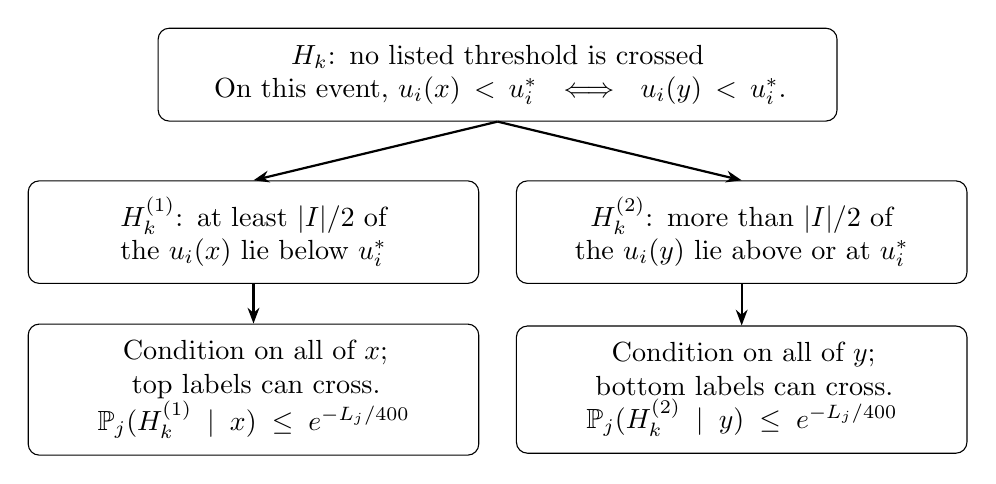
\begin{tikzpicture}[
  box/.style={draw,rounded corners,align=center,text width=5.3cm,
              minimum height=1.1cm,inner sep=6pt},
  arr/.style={-{Stealth[length=2mm]},thick}]
\node[box,text width=8.2cm] (b) at (0,0)
 {$H_k$: no listed threshold is crossed\\
  On this event, $u_i(x)<u_i^*\iff u_i(y)<u_i^*$.};
\node[box] (x) at (-3.1,-2)
 {$H_k^{(1)}$: at least $|I|/2$ of the $u_i(x)$ lie below $u_i^*$};
\node[box] (y) at (3.1,-2)
 {$H_k^{(2)}$: more than $|I|/2$ of the $u_i(y)$ lie above or at $u_i^*$};
\node[box] (cx) at (-3.1,-4)
 {Condition on all of $x$;\\
  top labels can cross.\\
  $\mathbb P_j(H_k^{(1)}\mid x)\le e^{-L_j/400}$};
\node[box] (cy) at (3.1,-4)
 {Condition on all of $y$;\\
  bottom labels can cross.\\
  $\mathbb P_j(H_k^{(2)}\mid y)\le e^{-L_j/400}$};
\draw[arr] (b.south) -- (x.north);
\draw[arr] (b.south) -- (y.north);
\draw[arr] (x) -- (cx);
\draw[arr] (y) -- (cy);
\end{tikzpicture}
\caption{The two parts of the no-crossing event are small after
conditioning on complementary endpoints. Each estimate controls the
matching masked square sum in Lemma~\ref{lem:conditional-convolution}; no
simultaneous avoidance over all indices is required.}
\label{fig:conditioning}
\end{figure}


Outside $H_k$, at least one chosen coordinate crosses. All coordinates
are ordered, so \eqref{eq:ratio-crossing} and
\eqref{eq:crossing-intensity} give $R_{x,y}(k)\le e^{-L_j}$.
On $H_k$ the ratio is at most $1$. This proves
\eqref{eq:tail-ratio-bound} and the lemma.
\end{proof}

\subsection{Completion of the contradiction}

Apply Lemma~\ref{lem:conditional-convolution} to the labelled law
$\mathbb P_j$, with
\[
 K=K_j,\quad D=D_j,\quad a=1/j,\quad c=c_* =e^{-90}/2,
 \qquad \eta=e^{-L_j},\quad \delta=e^{-L_j/400}.
\]
Equations~\eqref{eq:full-convolution} and~\eqref{eq:ratio-minimum}
verify its algebraic assumptions.  The proof of
Lemma~\ref{lem:truncation-bound} supplies the event of mass at least
$c_*$ and all central-coefficient bounds for sufficiently large $j$.
Lemma~\ref{lem:tail-attenuation} gives the tail estimate with conditional
probabilities under the full law.  Consequently
\[
 c_*\varepsilon_j
 \le(2K_j+1)\bigl(e^{-L_j}+2e^{-L_j/800}\bigr)
 \le\frac{\varepsilon_j}{j},
\]
where the last inequality is the parameter choice
\eqref{eq:polynomial}.  Since $\varepsilon_j>0$ and eventually
$1/j<c_*$, this is impossible.  This proves
Theorem~\ref{thm:measurable}.

\section{A continuous weight with one zero}
\label{sec:continuity}

The measurable obstruction of Theorem~\ref{thm:measurable} is now in place.
We will replace its logarithmic cost $g_*$ by a function continuous off one
point and tending to infinity at that point.  The replacement changes the
cost by the constant $1$ plus a measurable coboundary.  Since its transfer function need not be
bounded, we begin with the precise operator statement that will preserve
the obstruction.

\subsection{Transport by an affiliated positive operator}

A positive self-adjoint operator is \emph{affiliated} with a von Neumann
algebra if all its spectral projections belong to that algebra.  Such an
operator commutes, including on its domain, with every unitary in the
commutant.
The action of an invertible affiliated operator on projection lattices
also appears in \citet[Proposition~3.1]{mori}.  The form needed here
includes a specified intertwining domain and preservation of the trace;
we give a direct spectral-cutoff proof.

\begin{lemma}\label{lem:affiliated-transport}
Let $(\mathcal M,\tau)$ be a finite von Neumann algebra acting on a Hilbert
space, with faithful normal tracial state $\tau$.  Let $H$ be an injective
positive self-adjoint operator affiliated with $\mathcal M$, and let
$A,B\in\mathcal M$.  Suppose
\[
 A(\operatorname{Dom}H)\subseteq\operatorname{Dom}H,
 \qquad HA\zeta=BH\zeta\quad(\zeta\in\operatorname{Dom}H).
\]
For every projection $p\in\mathcal M$ with $A\operatorname{ran}p\subseteq
\operatorname{ran}p$, the projection $P$ onto
\[
 \overline{H(\operatorname{ran}p\cap\operatorname{Dom}H)}
\]
belongs to $\mathcal M$, is invariant under $B$, and satisfies
$\tau(P)=\tau(p)$.
\end{lemma}

\begin{proof}
Every commutant unitary preserves $\operatorname{ran}p$ and
$\operatorname{Dom}H$, and commutes with $H$ on that domain.  It therefore
maps the displayed closed space onto itself.  Its projection commutes with
the commutant, proving $P\in\mathcal M$.  If
$\zeta\in\operatorname{ran}p\cap\operatorname{Dom}H$, both invariance
assumptions give
$A\zeta\in\operatorname{ran}p\cap\operatorname{Dom}H$, and
$BH\zeta=HA\zeta$.  Thus $B$ preserves the unclosed image and, by
boundedness, its closure.

It remains to prove the trace assertion; bounded similarity cannot be
assumed.  Put $E_N=\mathbf1_{[1/N,N]}(H)$.  Since $H$ is injective,
$E_N\uparrow1$.  For $q_N=p\wedge E_N$, the bounded element $Hq_N=(HE_N)q_N$ of
$\mathcal M$ is bounded below by $1/N$ on its initial space.  Its image is
closed, and its polar decomposition identifies the initial projection
$q_N$ with its final projection, which is dominated by $P$.  Therefore
\[
 \tau(P)\ge\tau(p\wedge E_N)
 \ge\tau(p)+\tau(E_N)-1.
\]
The last inequality follows directly from the polar decomposition of
$(1-E_N)p$: its initial support is $p-(p\wedge E_N)$ and its final support
is at most $1-E_N$.  Letting $N$ increase gives $\tau(P)\ge\tau(p)$.

For the reverse inequality, set $q'_N=(1-p)\wedge E_N$.  The bounded
operator $H^{-1}q'_N=(H^{-1}E_N)q'_N$ is likewise bounded below on its initial space and
has closed image.  This image is orthogonal to $\operatorname{ran}P$.
Indeed, for $\eta\in\operatorname{ran}q'_N$ and
$\zeta\in\operatorname{ran}p\cap\operatorname{Dom}H$, self-adjointness
gives
\[
 \langle H^{-1}\eta,H\zeta\rangle=\langle\eta,\zeta\rangle=0;
\]
here $H^{-1}\eta$ lies in $\operatorname{Dom}H$.  Polar decomposition and
the same meet estimate yield
\[
 \tau(1-P)\ge\tau((1-p)\wedge E_N)
 \ge\tau(1-p)+\tau(E_N)-1.
\]
Passing to the limit proves the opposite inequality for $\tau(P)$.
\end{proof}

\subsection{Smoothing and moving the logarithmic drops}

We claim that there exist a nonnegative function $g$, finite and continuous
on $X\setminus\{0\}$ and tending to infinity at $0$, and an almost
everywhere finite real measurable function $b$ such that
\begin{equation}\label{eq:continuous-coboundary}
 g=g_*+1+b\circ\sigma-b\quad\text{almost everywhere},
 \qquad \int_Xg\,d\mu=\infty.
\end{equation}
The construction has three parts: smooth each drop, move its support into
a shrinking arc, and add an integrable background cost that guarantees
divergence at the center of those arcs.  Apart from the constant $1$, all changes will be explicit
coboundaries.

Fix $i\in J_j$ and put $\delta_i=\alpha_i/4$.  For $u\in X$, define the
continuous periodic smoothing of the sawtooth by
\[
 s_i(u)=\frac1{2\delta_i}\int_{-\delta_i}^{\delta_i}\{u+t\}\,dt.
\]
It equals $\{u\}$ outside the $\delta_i$-neighborhood of the cut at $0$.
Set
\[
 h_i(x)=C_j\bigl(\alpha_i+s_i(u_i(x))
                         -s_i(u_i(x)+\alpha_i)\bigr).
\]
The elementary identity
$\lfloor\{u\}+\alpha_i\rfloor=
\alpha_i+\{u\}-\{u+\alpha_i\}$ shows that $h_i$ is the corresponding
average of the original one-coordinate cost.  It is nonnegative and
continuous, with
\begin{equation}\label{eq:smoothed-support}
 \int_X h_i\,d\mu=C_j\alpha_i,
 \qquad \mu(\operatorname{supp}h_i)\le\alpha_i+2\delta_i.
\end{equation}
For
\[
 d_i^{\rm sm}(x)=C_j\bigl(s_i(u_i(x))-u_i(x)\bigr),
\]
we have the exact measurable identity
\begin{equation}\label{eq:smoothing-coboundary}
 h_i(x)=C_j\lfloor u_i(x)+\alpha_i\rfloor
                  +d_i^{\rm sm}(x)-d_i^{\rm sm}(\sigma x).
\end{equation}
The support of $d_i^{\rm sm}$ has measure at most $2\delta_i$.

Recall the shrinking arcs $O_j$, the integers $h_j^*$, and the continuous
partition of unity $\phi_{j,n}$, $0\le n\le h_j^*$, prepared in the
parameter construction, with
$\sigma^n(\operatorname{supp}\phi_{j,n})\subset O_j$.  Define
\[
 h'_i(x)=\sum_{n=0}^{h_j^*}(h_i\phi_{j,n})(\sigma^{-n}x).
\]
This is continuous and nonnegative, supported in $O_j$, and has the same
integral as $h_i$.  Telescoping gives
\begin{equation}\label{eq:relocation-coboundary}
 h'_i=h_i+d'_i-d'_i\circ\sigma,
 \qquad
 d'_i(x)=\sum_{n=1}^{h_j^*}\sum_{r=1}^n
                      (h_i\phi_{j,n})(\sigma^{-r}x).
\end{equation}
Although this transfer contains a double sum, its support is contained in
just $h_j^*$ translates of $\operatorname{supp}h_i$, one for each possible
$r$.  Consequently
\[
 \sum_i\left(\mu\{d_i^{\rm sm}\ne0\}+\mu\{d'_i\ne0\}\right)
 \le C\sum_j\frac{1+h_j^*}{K_j}<\infty.
\]
Thus each of the transfer sums has only finitely many nonzero terms
almost everywhere, including at the translated point $\sigma x$.

The sum $\sum_i h'_i$ is locally finite on $X\setminus\{0\}$ because its
successive blocks are supported in $O_j\downarrow\{0\}$.  It is therefore
continuous there.  Its integral is infinite: Tonelli's theorem and
$\alpha_i>1/(m_jK_j)$ give
\begin{equation}\label{eq:infinite-cost-integral}
 \int_X\sum_i h'_i\,d\mu
 =\sum_j C_j\sum_{i\in J_j}\alpha_i
 \ge\sum_j C_j/K_j=\infty,
\end{equation}
since $C_j\ge K_j^2$.  Local finiteness alone need not force divergence
at $0$; the following background supplies that remaining property.

\subsection{A background cost diverging at the zero}

Let $W_j=2^{j+1}$.  Choose continuous functions $0\le v_j\le1$ with
$v_j(0)=1$, supported in closed arcs $I_j$ shrinking to $\{0\}$.  Choose
these arcs small enough that $\sigma I_j,\ldots,\sigma^{W_j}I_j$ are
pairwise disjoint and
\[
 \sum_j W_j\mu(I_j)<\infty.
\]
This is possible because each finite set of distinct points
$\theta,2\theta,\ldots,W_j\theta$ has positive minimum separation.
For $x\ne0$, put
\[
 g_0(x)=1+\sum_j\left(v_j(x)-\frac1{W_j}
                              \sum_{n=1}^{W_j}v_j(\sigma^{-n}x)\right).
\]
For each $j$, disjointness bounds the norm of the subtracted function by
$1/W_j$.  These bounds sum to $1/2$, so the negative series converges
uniformly.  The positive series is locally finite away from $0$.
Consequently $g_0$ is continuous there and $g_0\ge1/2$.  For every fixed
integer $J$, the finite sum $\sum_{j\le J}v_j(x)$ tends to $J$ as $x\to0$.
The bounded negative series therefore implies $g_0(x)\to\infty$ as
$x\to0$.  Its integral is finite, since
$\sum_j\int v_j\,d\mu\le\sum_j\mu(I_j)<\infty$ and the negative series
is uniformly bounded.

Define
\[
 b_0(x)=\sum_j\frac1{W_j}\sum_{n=1}^{W_j}\sum_{r=1}^n
                                      v_j(\sigma^{-r}x).
\]
The $j$th summand is supported in $\bigcup_{r=1}^{W_j}\sigma^r I_j$.
The assumed summability makes this sum finite almost everywhere.  On a
conull set where the sums at $x$ and $\sigma x$ are finite, telescoping
shows
\[
 g_0=1+b_0\circ\sigma-b_0.
\]
Now let
\[
 g(x)=g_0(x)+\sum_i h'_i(x)\quad(x\ne0),\qquad g(0)=\infty,
 \qquad b=b_0-\sum_i(d_i^{\rm sm}+d'_i).
\]
The preceding arguments prove that $g$ is nonnegative, finite and
continuous off $0$, tends to infinity at $0$, and has infinite integral.
The transfer $b$ is real and finite almost everywhere.  Summing
\eqref{eq:smoothing-coboundary} and \eqref{eq:relocation-coboundary} is
legitimate on the common conull set where the transfer sums and the
original cost have finitely many nonzero terms.  Together with the
background identity this proves \eqref{eq:continuous-coboundary}.

\subsection{Conclusion and spectral consequences}

Define the function on the unit circle by
\[
 f(e^{2\pi i x})=e^{-g(x)},\qquad e^{-\infty}=0.
\]
It is continuous, is positive away from $1$, and vanishes at $1$.
Its modulus is nonconstant and its zero set has Haar measure zero.  Moreover,
\begin{equation}\label{eq:zero-log-integral}
 \int_{\mathbb T}\log f\,dm=-\infty.
\end{equation}
In particular, its Fuglede--Kadison determinant is zero
\cite{fuglede-kadison}: the spectral distribution of $\pi(f)$ is the
Haar distribution of $f$, so the determinant definition is precisely the
exponential of \eqref{eq:zero-log-integral}.  Also $|U\pi(f)|=\pi(f)$,
which gives the same determinant for $T_f=U\pi(f)$.  This conclusion uses
the nonnegative integral calculation \eqref{eq:infinite-cost-integral};
it does not require the transfer $b$ to be integrable.

Choose a finite Borel version of $b$ and discard all integer translates
of the null set where the coboundary identity fails.
Let $H_b$ be multiplication on the $k$th fiber coordinate by
$e^{b(\sigma^k x)}$, with its natural square-integrability domain.  It is
positive, self-adjoint, and injective.  Its spectral projections are
$\pi$-images of spectral indicators of $e^b$, hence lie in $M$.  Thus
$H_b$ is affiliated with $M$.  The coboundary identity gives the pointwise
factor equality
\[
 e^{b(\sigma^{k+1}x)}e^{-g(\sigma^k x)}
       =e^{-1}f_*(\sigma^k x)e^{b(\sigma^k x)}.
\]
For every $\zeta\in\operatorname{Dom}H_b$, the right-hand side defines
the $k+1$ coordinate of $e^{-1}T_*H_b\zeta$, a square-integrable vector
because $T_*$ is bounded.  Therefore
\[
 T_f\zeta\in\operatorname{Dom}H_b,
 \qquad H_bT_f\zeta=e^{-1}T_*H_b\zeta.
\]
Lemma~\ref{lem:affiliated-transport} sends any invariant projection of
$T_f$ to an invariant projection of $e^{-1}T_*$ having the same trace.
Multiplication by the nonzero scalar $e^{-1}$ does not change invariant
ranges.  Theorem~\ref{thm:measurable} therefore excludes traces strictly
between $0$ and $1$.  This proves Theorem~\ref{thm:main} for the arbitrary
irrational $\theta$ fixed at the start.

The same continuous weight has a stronger spectral property, which we
record with an elementary proof.  This is the zero-determinant case of
\citet[Theorem~2.3]{zfs}.  We include the truncated-logarithm argument,
which uses uniform averaging under irrational rotation.

\begin{corollary}\label{cor:quasinilpotent}
The constructed operator $T_f$ is nonzero and quasinilpotent.
\end{corollary}

\begin{proof}
For $M>0$, the function
$\ell_M(x)=\log\max(f(e^{2\pi i x}),e^{-M})$ is continuous.
Its integrals decrease to $-\infty$ by
\eqref{eq:zero-log-integral}.  Irrational rotation averages of a continuous
function converge uniformly to its integral: this follows for Fourier
monomials from their geometric sums and then for continuous functions by
uniform trigonometric approximation.  Hence, for any $a>0$, first choosing
$M$ with $\int_X\ell_M\,d\mu<-2a$ and then taking $n$ sufficiently large
gives
\[
 \sup_{x\in X}\prod_{k=0}^{n-1}f(e^{2\pi i\sigma^k x})
 \le\sup_{x\in X}\exp\left(\sum_{k=0}^{n-1}\ell_M(\sigma^k x)\right)
 \le e^{-an}.
\]
The expression on the left is $\|T_f^n\|$, because the power is a unitary
$U^n$ times multiplication by that continuous product.  The spectral-radius
formula yields radius zero, since $a$ was arbitrary.  Finally $T_f\ne0$
because $f>0$ almost everywhere.
\end{proof}

\appendix
\section{A product-rotation realization}\label{p:sec:product}

The circle proof replaces independent coordinates by divisible characters
and ordered digits.  On a countable product of circles, independence is
available directly.  This gives a different sampling result: prescribed
triangular laws in any finite set of coordinates are weak limits of
positive orbit-pair measures, with both marginal densities uniformly
bounded in $L^2$.  We prove that result and use it to construct a second
concrete model for the convolution obstruction.

All notation in this appendix is local.  Let
\[
 X=\T^{\N},\qquad \T=\R/\Z,
\]
with product Haar probability $\mu$ and its compact metrizable product
topology.  Coordinates are represented in $[0,1)$, and $x\le y$ means
$x_i\le y_i$ for every $i$.  This order is Borel; its graph need not be
closed at the circle cuts.  For a sequence of angles $\theta=(\theta_i)$,
write $\sigma_\theta x=x+\theta$.  On
$\mathcal H=L^2(X,\mu;\ell^2(\Z))$, put
\[
 (\pi(a)\zeta)(x)_k=a(\sigma_\theta^k x)\zeta(x)_k,
 \qquad (U\zeta)(x)=S\zeta(x),\qquad Se_k=e_{k+1},
\]
and let $M=W^*(U,\pi(L^\infty(X)))$.

\begin{theorem}[Product realization]\label{p:thm:model}
There are angles $0<\theta_i<1$ and costs $c_i>0$, with
$\sum_i\theta_i<\infty$ and $1,\theta_1,\theta_2,\ldots$ rationally
independent, such that the measurable weight
\[
 f(x)=\exp\left(-\sum_{i\ge1}c_i\lfloor x_i+\theta_i\rfloor\right)
\]
is positive almost everywhere and has $\int_X\log f\,d\mu=-\infty$.
The algebra $M$ is a type $\mathrm{II}_1$ factor with separable predual,
and $T=U\pi(f)$ is nonzero and norm-quasinilpotent, with
$\Delta(T)=0$.  Every projection $p\in M$ satisfying $(1-p)Tp=0$ is
$0$ or $1$.

Moreover, $|T|$ has pure-point spectral type.  The abelian algebra
generated by any finite family of polar conjugates
$U^n|T|U^{-n}$ is atomic, whereas
$W^*(U^n|T|U^{-n}:n\in\Z)$ is diffuse.
\end{theorem}

The last statement concerns spectral type: it does not require every
point of the spectrum of $|T|$ to be an eigenvalue.  In particular, zero
can be a spectral accumulation point although $f>0$ almost everywhere.
As in the principal construction, the absence of invariant projections
refers to the specified containing factor.  For instance, the subspaces
$L^2(X,\mu;\overline{\operatorname{span}}\{e_k:k\ge m\})$ are
invariant under the represented forward weighted shift, but their
constant-field projections do not satisfy the covariance required for
membership in $M$.

The proof has three product-specific tasks.  We first choose angles for
which the finite-coordinate sampling theorem holds.  We then pass the invariant
projection identity from those measures to biased product couplings.
Finally we verify the positive-event and tail-attenuation hypotheses of
Lemma~\ref{lem:conditional-convolution}.  The field decomposition,
compact-set transfer, and scalar sampling and density estimates are the
lemmas already proved in the main text; no part of this appendix is
needed for the prescribed-angle theorem.

\subsection{Scales and independent angles}\label{p:sec:scales}

We choose the finite polynomial accuracy before choosing each new block.
This leaves enough freedom to obtain both the sampling estimates and the
threshold crossings needed by Lemma~\ref{lem:conditional-convolution}.
All choices in this subsection are independent of any invariant projection.

Partition $\N=\{1,2,\ldots\}$ into consecutive finite blocks $J_j$ of
length $m_j$, writing
\[
 d_0=0,\qquad d_j=\sum_{s\le j}m_s,\qquad
 J_j=\{d_{j-1}+1,\ldots,d_j\}.
\]
The cutoff $K_j$ will specify the finite coefficient window in the
contradiction, while $D_j$ and $\varepsilon_j$ will give the coefficient
bound and the product lower bound from Lemma~\ref{lem:polynomial-coefficient}.  After these
are fixed, $L_j$ specifies the required decay of the omitted terms;
the logarithmic drop $C_j$ and the block length $m_j$ are chosen to
achieve that decay while retaining uniform bounds on the coupling
marginals.

We now choose these parameters.  Put $\kappa_j=1/(100j)$ and
start with $K_1=100$ and $G_1=1$.  At stage $j$, the numbers $K_j,G_j$
and all parameters of earlier blocks have already been fixed.  Make
the following choices in the stated order.

\begin{enumerate}
\item Define
\[
 D_j=\exp\left((K_j+1)\sum_{s<j}C_sm_s\right).
\]
Apply Lemma~\ref{lem:polynomial-coefficient} with $K=K_j$, $D=D_j$, and
$\delta=1/j$ to choose $\varepsilon_j>0$.  This is possible because
$D_j\ge1\ge1/j$.  Consequently,
\begin{equation}\label{p:eq:poly-lower}
 \max_{0\le n\le2K_j}|(AB)_{-n}|\ge\varepsilon_j
\end{equation}
whenever $A,B$ are supported in $[-K_j,K_j]$, their coefficients
have modulus at most $D_j$, and $|A_0|,|B_0|\ge1/j$.

\item Choose $L_j\ge1$, increasing with $j$, so large that
\begin{equation}\label{p:eq:epsilon-choice}
 (2K_j+1)3\exp(-L_j/10000)\le\frac{\varepsilon_j}{j}.
\end{equation}
Set $C_j=\max\{L_j,K_j^2\}$, and choose a finite $G_{j+1}\ge1$
such that
\begin{equation}\label{p:eq:G-choice}
 \kappa_{j+1}\sqrt{G_{j+1}}\ge L_j.
\end{equation}

\item Choose an integer $m=m_j$ sufficiently large, and set
\[
 K_{j+1}=\left\lceil m^{(3/4)m}\right\rceil,
\]
subject to
\begin{equation}\label{p:eq:scale-conditions}
 \begin{gathered}
 m\ge\max\{K_j,2^j,4G_j,100\},\qquad d_{j-1}\le m/100,\\
 \kappa_jm^{1/40}\ge L_j,\qquad
 G_{j+1}K_{j+1}<m^{(4/5)m}.
 \end{gathered}
\end{equation}
\end{enumerate}

Every choice is finite and feasible.  Indeed, the first two steps do
not depend on the new $m_j$.  All but the final requirement in
\eqref{p:eq:scale-conditions} are lower bounds on $m$.  For the final
one, the already fixed number $G_{j+1}$ satisfies
\[
 \frac{G_{j+1}\lceil m^{(3/4)m}\rceil}{m^{(4/5)m}}
 \le 2G_{j+1}m^{-m/20}\longrightarrow0.
\]
There is therefore no upper restriction conflicting with the lower
bounds.

Write
\begin{equation}\label{p:eq:N-and-widths}
 N_j=m_jK_j,\qquad a_j=G_j/m_j,\qquad b_j=m_j^{-19/20}.
\end{equation}
The construction gives the useful consequences
\begin{equation}\label{p:eq:scale-consequences}
 \begin{gathered}
 m_j\ge2^j,\qquad d_j\le1.01m_j,\qquad N_j\le m_j^2,\\
 K_{j+1}>2K_j,\qquad
 \sum_{s>j}\frac1{K_s}\le\frac2{K_{j+1}},\qquad
 \frac1{m_j}\le a_j,b_j\le\frac14.
 \end{gathered}
\end{equation}
For example, $m_j\ge100$ and $m_j\ge K_j$ imply
$K_{j+1}\ge m_j^{(3/4)m_j}>2m_j\ge2K_j$, and the reciprocal
estimate follows by summing a geometric majorant.  Also
$m_{j+1}\ge K_{j+1}>m_j$, so each of $m_j,K_j,N_j$ is increasing.
The upper bound for $a_j$ follows from $m_j\ge4G_j$; the other width
bounds follow from $G_j\ge1$ and $m_j\ge100$.

Use the coordinate order on $X$ defined above.

On a separate product probability space choose independent random
angles $\theta_i$, with $\theta_i$ uniform on $[1/N_j,2/N_j]$ when
$i\in J_j$, and let
\[
 \sigma_\theta x=x+\theta\quad\text{in }X.
\]
For every realization,
\begin{equation}\label{p:eq:angle-summability}
 \sum_{i=1}^\infty\theta_i
 \le2\sum_{j=1}^\infty\frac{m_j}{N_j}
 =2\sum_{j=1}^\infty\frac1{K_j}<\infty.
\end{equation}
Almost surely $1,\theta_1,\theta_2,\ldots$ are rationally independent.
To see this, multiply any proposed finite rational relation by a
common denominator.  If some angle has a nonzero integer coefficient,
conditioning on all other angles leaves one prescribed value of an
atomless random variable, an event of probability zero.  A relation
with no angle term cannot hold unless its constant term is zero.
There are only countably many nontrivial finite integer relations.

For a rationally independent realization the rotation is ergodic
and free.  Indeed, the characters
\[
 x\longmapsto\exp\left(2\pi i\sum_i v_ix_i\right),
 \qquad v_i\in\Z,\quad v_i=0\text{ for all but finitely many }i,
\]
form an orthonormal basis of $L^2(\mu)$: finite-coordinate functions
are dense, and the usual Fourier bases are complete on each finite
torus.  Translation multiplies this character by
$\exp(2\pi i\sum_i v_i\theta_i)$, which equals $1$ only for the
constant character.  Hence the invariant $L^2$ functions are constant,
which is ergodicity.  Also $n\theta_1\notin\Z$ for every
$n\in\Z\setminus\{0\}$, so $\sigma_\theta^n x\ne x$ for every
$x\in X$.

\begin{proposition}[Phase ranges]\label{p:prop:phases}
Almost surely, for every sufficiently large $j$ the following hold
simultaneously for all integers $k$ in the indicated ranges, with
$m=m_j$:
\begin{enumerate}
\item If $G_jK_j\le |k|\le N_j/4$, then every $i\in J_j$ satisfies
\[
 1-\{k\theta_i\}\in[a_j,1-a_j].
\]
\item If $N_j/4\le |k|\le m^{(4/5)m}$, then at least $m/20$
coordinates $i\in J_j$ satisfy
\[
 1-\{k\theta_i\}\in[b_j,1-b_j].
\]
\end{enumerate}
The first assertion in fact holds at every stage and for every
realization of the angles in their prescribed intervals.
\end{proposition}

\begin{proof}
In the first range, put $t=|k|\theta_i$.  The angle bounds give
\[
 a_j=G_j/m_j\le t\le1/2.
\]
For $k>0$ the threshold is $1-t$, and for $k<0$ it is $t$.
Both belong to $[a_j,1-a_j]$ because $a_j\le1/4$.

For the second range, the uniform law of $k\theta_i$ on an interval
of length $|k|/N_j$ has, after reduction modulo one, a density bounded
by
\[
 1+N_j/|k|\le5.
\]
This follows by counting the integer translates covering a point:
the covering multiplicity of an interval of length $r$ is at most
$r+1$.  The statement also applies to negative $k$ by reflection.
Thus a given coordinate misses $[b_j,1-b_j]$ with probability at
most $10b_j$.  If fewer than $m/20$ coordinates satisfy the assertion,
more than $19m/20$ coordinates miss the interval.  Independence over
$i\in J_j$ and a union bound over the possible sets of misses show
that, for a fixed $k$, this failure probability is at most
$2^m(10b_j)^{(19/20)m}$ for large $m$.  A further union bound over
the at most $2m^{(4/5)m}$ nonzero integers in the range gives
\[
 \mathbb P(\text{failure at stage }j)
 \le2m^{(4/5)m}2^m(10b_j)^{(19/20)m}
 =\exp\left(-\frac{41}{400}m\log m+O(m)\right).
\]
These probabilities are summable because $m_j\ge2^j$.
The first Borel--Cantelli Lemma now gives the second assertion for
all sufficiently large $j$, simultaneously for every integer in
each stated range.
\end{proof}

We retain the random angles until the sampling construction below
has supplied one further probability-one property.

\subsection{Sampling ordered orbit pairs}\label{p:sec:sampling}

We next approximate prescribed changes in finitely many coordinates by
positive orbit moves.  Both endpoint distributions must remain controlled:
this will allow the projection identity to pass from orbit pairs to the
couplings used in the product construction.  The scalar estimates of
Lemma~\ref{lem:scalar-sampling-estimates} apply coordinate by coordinate;
we prove here the growing-product estimate and the ordered weak limit.

The coordinate order is only Borel in the product-circle topology:
already in one circle, the ordered pairs $(1/2,1-1/n)$ converge to
the unordered pair $(1/2,0)$.  Thus the closed-relation hypothesis in
the classical coupling theorem \cite[Corollary~3.2]{Edwards1978} does
not apply directly.  The result below also requires approximating
measures supported on positive orbit pairs, with both marginal densities
controlled; those are additional conclusions proved by the sampling
construction.

For a finite set $I\subset\N$, define a finite Borel measure
$\lambda_I$ on $X\times X$ as follows.  In each coordinate $i\in I$
use the unnormalized triangular measure
\[
 \ind_{\{0\le x_i<y_i<1\}}\,dx_i\,dy_i,
\]
and in each other coordinate use the law of $(x_i,x_i)$ for uniform
$x_i\in[0,1)$.  Take the product over all coordinates.  Equivalently,
one can first normalize the finitely many triangular factors and
then multiply the resulting probability measure by $2^{-|I|}$.
In particular,
\[
 \lambda_I(X\times X)=2^{-|I|}.
\]
Its two marginal densities relative to $\mu$ are, respectively,
$\prod_{i\in I}(1-x_i)$ and $\prod_{i\in I}y_i$; they are bounded
by $1$.  The measure is carried by $x\le y$.

\begin{proposition}[Ordered orbit-pair sampling]\label{p:prop:sampling}
With probability one in the choice of $\theta$, the following holds
for every finite $I\subset\N$.  There are positive finite Borel
measures $\eta_{I,l}$ on $X\times X$ converging weakly to
$\lambda_I$, each carried by ordered pairs of the form
\[
 (x,y)=(x,\sigma_\theta^n x)
\]
with $n$ in a finite set of positive integers.  Both marginals of
$\eta_{I,l}$ have $L^2(\mu)$ densities, and their $L^2$ norms are
bounded uniformly in $l$.  The bound may depend on $I$ and on the
fixed realization of $\theta$.  Weak convergence here means
convergence against every continuous function on the compact space
$X\times X$.
\end{proposition}

\begin{proof}
We give the construction and its estimates before choosing the
probability-one event.  The notation $O(\cdot)$ in this proof has
absolute constants, uniform in the coordinate, the selected powers,
and the interval endpoints involved in a rectangle test.

We average many separated orbit powers so that both marginal densities
approach those of an ideal model with independent uniform phases.  The
coordinate weights impose triangular laws on $I$ and concentrate near
the diagonal elsewhere, while their marginal bounds remain uniform in
the growing product.  A final restriction to ordered tail coordinates
removes asymptotically negligible mass.

\paragraph{Separated powers and phase discrepancy}

Take $l$ sufficiently large that $m_l\ge200$, as required by the scalar
lemma. At stage $l$ write $m=m_l$, $d=d_l$, and set
\[
 Q=m^{(7/10)m},\qquad H=m^{300},\qquad R=N_lm^{1000}.
\]
For all sufficiently large $l$ we can choose, deterministically, a
set $\mathcal N_l$ of integers in $[Q/2,Q]$ such that
\begin{equation}\label{p:eq:sampling-separation}
 \begin{gathered}
 P_l:=|\mathcal N_l|\ge m^{0.69m},\\
 |vn+v'n'|>R\quad
 \left(\begin{array}{l}
 n,n'\in\mathcal N_l,\ n\ne n',\\
 v,v'\in\Z,\ |v|,|v'|\le H,\ (v,v')\ne(0,0)
 \end{array}\right).
 \end{gathered}
\end{equation}
Indeed, given a previously selected $n$, a fixed frequency pair with
$v'\ne0$ forbids an interval of possible $n'$ of length
$2R/|v'|\le2R$, hence at most $2R+2$ integers.  There are
$O(H^2)$ frequency pairs.  Since $N_l\le m^2$, each selection
therefore excludes at most $O(m^{1602})$ integers.  When $v'=0$
and $v\ne0$, the inequality is automatic because $n\ge Q/2>R$
eventually; likewise, a zero first frequency creates no obstruction.
The constraints are symmetric in the selected powers, since the
full set of frequency pairs is used.  Greedy selection from the
$\asymp Q$ available integers yields at least
$cQ/m^{1602}\ge m^{0.69m}$ choices for large $m$.

For a coordinate $i\in J_s$ with $s\le l$, the angle $\theta_i$ is
uniform on $[1/N_s,2/N_s]$.  Apply the separated-phase part of
Lemma~\ref{lem:scalar-sampling-estimates} with
\[
 N_0=N_s\le N_l=N\le m^2.
\]
The powers just selected satisfy its separation hypothesis.  Thus
$t_n=\{n\theta_i\}$ has a density $\varphi_{i,n}$ satisfying
\begin{equation}\label{p:eq:single-phase-density}
 \|\varphi_{i,n}-1\|_\infty\le N_s/n\le N_l/n.
\end{equation}
In particular, that density is at most two for large $l$.  For distinct
selected powers and functions $g,g'$ of bounded variation, the same
lemma gives
\begin{equation}\label{p:eq:bv-discrepancy}
 \begin{split}
 \left|\mathbb E_\theta g(t_n)g'(t_{n'})
       -\left(\int_0^1g\right)\left(\int_0^1g'\right)\right|
 &\le c m^{-80}
   (\|g\|_\infty+\operatorname{Var}g)
   (\|g'\|_\infty+\operatorname{Var}g').
 \end{split}
\end{equation}
No independence between $t_n$ and $t_{n'}$ is asserted.  The imported
estimate uses their Fourier coefficients and one-dimensional marginal
densities, and so applies even when their joint law is singular.
We shall also use the direct consequence of
\eqref{p:eq:single-phase-density}
\begin{equation}\label{p:eq:single-phase-test}
 \left|\mathbb E_\theta g(t_n)-\int_0^1g(t)\,dt\right|
 \le\frac{N_l}{n}\int_0^1|g(t)|\,dt.
\end{equation}

\paragraph{The weighted measures and both marginal orientations}

Fix a finite $I$ and restrict to sufficiently large $l$ that
$I\subset\{1,\ldots,d\}$.  Set
\[
 h=m^{-3/5},\qquad \Delta(s)=\min(s,1-s),\qquad \alpha=m^{-2}.
\]
For $0\le s,t<1$ define
\begin{equation}\label{p:eq:sampling-weights}
 w_i(s,t)=
 \begin{cases}
 \ind_{\{0<t<1-s\}},&i\in I,\\[1mm]
 \displaystyle\ind_{\{\Delta(s)\ge\alpha\}}
 \frac{\ind_{\{0<t<h\Delta(s)\}}}{h\Delta(s)},&i\notin I.
 \end{cases}
\end{equation}
The second line is defined to be zero if $\Delta(s)<\alpha$.
Let $\widetilde\eta_{I,l}$ be the average, over $n\in\mathcal N_l$,
of the push-forward under $x\mapsto(x,\sigma_\theta^n x)$ of
\begin{equation}\label{p:eq:untrimmed-weight}
 W_n(x)\,d\mu(x),\qquad
 W_n(x)=\prod_{i\le d}w_i(x_i,\{n\theta_i\}).
\end{equation}
Each weight is bounded for fixed $l$, so these are finite positive
measures.  They are carried by pairs satisfying $x_i<y_i$ for $i\le d$, since
$h\Delta(x_i)\le h(1-x_i)<1-x_i$ and $h<1$.

We will treat the marginals both without a test and after restriction
to a cylinder rectangle
\[
 \mathcal R=\{(x,y):x_i\in E_i^x,\ y_i\in E_i^y
                         \text{ for every }i\},
\]
where the $E_i^x,E_i^y$ are intervals with rational endpoints and
all but finitely many are the whole circle.  Take $l$ large enough
that all tested coordinates are at most $d$.  A missing test is
represented by using the whole circle for every interval.  For the
first and second marginal, respectively, define
\begin{equation}\label{p:eq:oriented-weights}
 \begin{split}
 u_i^{(1)}(s,t)
 &=w_i(s,t)\ind_{E_i^x}(s)\ind_{E_i^y}(\{s+t\}),\\
 u_i^{(2)}(s,t)
 &=w_i(\{s-t\},t)\ind_{E_i^x}(\{s-t\})\ind_{E_i^y}(s).
 \end{split}
\end{equation}
Changing variables $y=\sigma_\theta^n x$ preserves Haar measure.
It follows that the two tested marginal densities are exactly the
averages of the products of the corresponding $u_i^{(r)}$.
There is no factor from coordinates past $d$, even in the second
orientation, since their unweighted Haar law is translation invariant.

We check the extra factors introduced by triangular laws and interval
tests.  Write $u_i$ for either orientation and put
\[
 \bar u_i(s)=\int_0^1u_i(s,t)\,dt,\qquad
 A_i=\int_0^1\bar u_i(s)^2\,ds.
\]
Uniformly in $s$, the coordinate, and the test intervals, we have
\begin{equation}\label{p:eq:weight-variation}
 \|u_i(s,\cdot)\|_\infty+
       \operatorname{Var}_t u_i(s,\cdot)
 =O(m^{13/5})=O(m^{10}).
\end{equation}
For an untested triangular factor, the bound is $O(1)$: in the first
orientation its support in $t$ is $0<t<1-s$, and in the second it is
$0<t\le s$.  The possible value at $t=s$ affects no integral.
For the untested near-diagonal factors,
Lemma~\ref{lem:scalar-sampling-estimates} gives the bound
$O(m^{13/5})$.  To include the tests, in either orientation the
extra factor is a constant in $\{0,1\}$ times an interval indicator
translated or reflected modulo one.  Its supremum is at most one
and its variation is bounded by an absolute constant.  The inequality
\[
 \operatorname{Var}(ab)\le
 \|a\|_\infty\operatorname{Var}(b)
 +\|b\|_\infty\operatorname{Var}(a)
\]
therefore proves \eqref{p:eq:weight-variation}, including all jumps at
the test endpoints.

The moment bounds needed below are
\begin{equation}\label{p:eq:one-coordinate-moments}
 0\le\bar u_i(s)\le2,\qquad
 0\le A_i\le1+O(h^2),\qquad
 \int_0^1\int_0^1u_i(s,t)^2\,ds\,dt
       =O(h^{-1}\log m).
\end{equation}
For an untested triangular factor the two averages are exactly $1-s$
and $s$, respectively.  In either orientation its total integral and
squared integral are $1/2$, while $A_i=1/3$.  For an untested
near-diagonal factor, Lemma~\ref{lem:scalar-sampling-estimates} gives
\[
 \|\bar u_i\|_\infty\le2,\qquad
 A_i\le1+\frac{h^2}{(1-h)^2},\qquad
 \iint u_i(s,t)^2\,ds\,dt=\frac2h\log\frac1{2\alpha}.
\]
Since tests only decrease the nonnegative factors and their averages,
these statements imply \eqref{p:eq:one-coordinate-moments} for every
tested factor.  Their actual masses need not agree; in particular,
the near-diagonal integral identities are not being imposed on the
triangular factors or on the tested kernels.  The quadratic error
$O(h^2)$ is what keeps the product of the moment bounds controlled as
the number of coordinates grows.

\paragraph{The estimate in the growing product dimension}

For either fixed orientation and a fixed rectangle test or no test,
write
\[
 \begin{aligned}
 q_n(z)&=\prod_{i\le d}u_i(z_i,\{n\theta_i\}),&
 Z_l(z)&=\frac1{P_l}\sum_{n\in\mathcal N_l}q_n(z),\\
 Z_l^0(z)&=\prod_{i\le d}\bar u_i(z_i),&
 A&=\prod_{i\le d}A_i=\|Z_l^0\|_2^2.
 \end{aligned}
\]
We prove the estimate
\begin{equation}\label{p:eq:sampling-L2}
 \mathbb E_\theta\|Z_l-Z_l^0\|_{L^2(\mu)}^2
 \le O(dm^{-40})+\frac{(c h^{-1}\log m)^d}{P_l}.
\end{equation}
The independence used here is independence across coordinates
$\theta_i$.  In a single coordinate two phases may still be
dependent, as already accounted for in \eqref{p:eq:bv-discrepancy}.

For distinct $n,n'$, Tonelli's Theorem, product Haar measure, and
coordinate independence yield the exact factorization
\[
 \mathbb E_\theta\langle q_n,q_{n'}\rangle
 =\prod_{i\le d}\int_0^1
   \mathbb E_\theta\bigl[
    u_i(s,\{n\theta_i\})u_i(s,\{n'\theta_i\})\bigr]\,ds.
\]
By \eqref{p:eq:weight-variation} and \eqref{p:eq:bv-discrepancy}, its
$i$th factor is $A_i+e_i$ with $|e_i|\le c m^{-50}$.
Similarly,
\[
 \mathbb E_\theta\langle q_n,Z_l^0\rangle
 =\prod_{i\le d}\int_0^1
       \bar u_i(s)\mathbb E_\theta u_i(s,\{n\theta_i\})\,ds.
\]
Here \eqref{p:eq:single-phase-test} and $\bar u_i\le2$ bound the
error in each factor from $A_i$ by $4N_l/n=O(m^{-50})$.
Thus both sorts of factors have the same stated error bound.

The product errors do not require any lower bound on $A_i$.
Telescoping gives
\begin{equation}\label{p:eq:sampling-product-error}
 \left|\prod_{i\le d}(A_i+e_i)-\prod_{i\le d}A_i\right|
 \le cdm^{-50}(1+ch^2+cm^{-50})^{d-1}
 =O(dm^{-50}),
\end{equation}
because \eqref{p:eq:scale-consequences} gives $d\le1.01m$, and hence
$dh^2\le1.01m^{-1/5}$.  In particular,
$A\le(1+ch^2)^d=O(1)$.

For a self-pairing, use only the one-phase density bound at most $2$
and \eqref{p:eq:one-coordinate-moments}:
\[
 \mathbb E_\theta\|q_n\|_2^2
 =\prod_{i\le d}\int_0^1
            \mathbb E_\theta u_i(s,\{n\theta_i\})^2\,ds
 \le(c h^{-1}\log m)^d.
\]
To see the cancellation of all other main terms explicitly, expand
the squared norm.  The distinct-pair terms have total averaging
weight $1-1/P_l$ and main term $(1-1/P_l)A$.  The cross terms with
$Z_l^0$ have main term $-2A$, and the final squared norm of $Z_l^0$
is $A$.  Their sum is $-A/P_l\le0$.  By
\eqref{p:eq:sampling-product-error}, their remaining contribution
has absolute value $O(dm^{-50})$.  The self-pairings have total
weight $1/P_l$.  Dropping $-A/P_l$ proves the slightly weaker
bound \eqref{p:eq:sampling-L2}.

This estimate is summable in $l$.  Indeed,
\[
 \log_m (c h^{-1}\log m)^d
 \le1.01m\left(\frac35+\log_m(c\log m)\right)
 \le0.65m
\]
for large $m$, whereas $P_l\ge m^{0.69m}$.  Thus
\begin{equation}\label{p:eq:sampling-summable}
 \mathbb E_\theta\|Z_l-Z_l^0\|_2^2
 \le O(m^{-39})+m^{-0.04m},
\end{equation}
whose sum is finite by $m_l\ge2^l$.

\paragraph{One probability-one event and the weak limit}

For each fixed finite $I$, orientation, and rational cylinder
rectangle or absent test, Tonelli's Theorem applied to
\eqref{p:eq:sampling-summable} shows that
\[
 \sum_l\|Z_l-Z_l^0\|_2^2<\infty
 \quad\text{almost surely},
\]
where only the sufficiently large admissible stages are included.
In particular, $\|Z_l-Z_l^0\|_2\to0$.  Finite subsets of $\N$
form a countable family, as do finite cylinder rectangles with
rational endpoints, and there are only two orientations.  Intersect
these countably many probability-one events.  For the remainder
of the proof take any $\theta$ in this intersection.

Without a test, $Z_l$ is a marginal density of
$\widetilde\eta_{I,l}$.  Since $\|Z_l^0\|_2^2=A=O(1)$, the
$L^2$ convergence just proved bounds both marginal norms uniformly
in $l$.  We may omit finitely many initial stages; alternatively,
each of their densities is bounded for fixed $l$, so they can be
included by enlarging the bound.  The total masses of
$\widetilde\eta_{I,l}$ are consequently uniformly bounded.

For a fixed cylinder rectangle $\mathcal R$, using the first
orientation with its test shows that
\[
 \left|\widetilde\eta_{I,l}(\mathcal R)
       -\int_X Z_l^0\,d\mu\right|
 \le\|Z_l-Z_l^0\|_2\longrightarrow0.
\]
The ideal integral has a direct product interpretation on the first
$d$ coordinates.  For $i\in I$, integration of $w_i(x_i,t)$ in
$x_i,t$ gives exactly the triangular measure under $y_i=x_i+t$.
For $i\notin I$, first take uniform $x_i$, discard
$\Delta(x_i)<\alpha$, and, otherwise, take $t$ uniform in
$(0,h\Delta(x_i))$, setting $y_i=x_i+t$.  Before the discard this
is a probability law (the value at the two endpoint values of
$x_i$ may be defined arbitrarily), and
$|y_i-x_i|\le h/2$.  The total loss caused by all cutoffs is at most
\[
 2d\alpha=2dm^{-2}\longrightarrow0,
\]
by the union bound, with the finite triangular factors having mass
at most one.  Each fixed tested coordinate outside $I$ therefore
converges to its uniform diagonal law.  More explicitly, outside
an $h$-neighborhood of a tested interval's endpoints, membership
of $y_i$ in that interval agrees with membership of $x_i$; the
neighborhood has Lebesgue measure $O(h)$.  Since a fixed rectangle
tests only finitely many coordinates, all such errors vanish.
Untested coordinates contribute only their masses, and the total
cutoff estimate controls their product even as $d$ increases.
It follows that
\begin{equation}\label{p:eq:sampling-rectangle-limit}
 \widetilde\eta_{I,l}(\mathcal R)\longrightarrow
                  \lambda_I(\mathcal R).
\end{equation}

These limits imply weak convergence on $X\times X$.  Here are the
topological details.  The boundaries of the interval rectangles
have zero $\lambda_I$ measure, since every single-coordinate
marginal of $\lambda_I$ is absolutely continuous.  Every continuous
function on the compact product can be uniformly approximated by
a continuous function of finitely many coordinates: in a summable
product metric, replace the tail coordinates by fixed points and
use uniform continuity.  On the resulting finite torus, a sufficiently
fine rational grid gives a step function, a finite linear combination
of rational rectangle indicators, with arbitrarily small uniform
error.  Thus \eqref{p:eq:sampling-rectangle-limit} and the uniform
bound on total masses give convergence of integrals for every
continuous function.  In particular,
\[
 \widetilde\eta_{I,l}\ \Longrightarrow\ \lambda_I.
\]

\paragraph{Trimming the tail to impose order everywhere}

The untrimmed measures now have the required weak limit and both
marginal bounds.  It remains to impose order past the first $d$
coordinates.  Define
$\eta_{I,l}$ by restricting $\widetilde\eta_{I,l}$ to the Borel
set where $x_i\le y_i$ also for every $i>d$.  For a fixed selected
$n$, the weight $W_n$ depends only on the first $d$ coordinates,
so the tail $x$-coordinates remain independent uniform coordinates
under that summand, apart from multiplication by its total mass.
For a uniform tail coordinate, the probability that
$x_i>\{x_i+n\theta_i\}$ is exactly $\{n\theta_i\}\le n\theta_i$.
Consequently, uniformly over $n\in\mathcal N_l$, the relative mass
discarded from this summand is at most
\begin{equation}\label{p:eq:sampling-tail-trim}
 \begin{split}
 \sum_{i>d}n\theta_i
 &\le 2m^{(7/10)m}\sum_{s>l}\frac1{K_s}\\
 &\le\frac{4m^{(7/10)m}}{K_{l+1}}
 \le4m^{-m/20}\longrightarrow0.
 \end{split}
\end{equation}
The union bound is valid for the countable tail by increasing
finite unions.  More precisely, the discarded mass of a summand
equals its total mass times the Haar probability of its tail
failure event, because the weight and that event depend on disjoint
coordinates.  This statement also holds for a summand of mass zero.
Averaging over $n$ shows that the total discarded mass is bounded
by \eqref{p:eq:sampling-tail-trim} times the uniformly bounded
untrimmed mass.  Hence the difference of the two measures tends
to zero in total variation and
$\eta_{I,l}\Longrightarrow\lambda_I$.

Each trimmed marginal is a submeasure of the corresponding
untrimmed marginal.  Its Radon--Nikodym density is therefore
nonnegative and bounded almost everywhere by the untrimmed density,
so its $L^2$ norm cannot increase.  Trimming preserves the finite
set of positive orbit powers and now imposes order in every
coordinate.  All conclusions hold on the single probability-one
event already constructed, for every finite $I$, proving the
Proposition.
\end{proof}

We now fix one realization $\theta$ for which rational independence,
Proposition~\ref{p:prop:phases}, and Proposition~\ref{p:prop:sampling}
all hold, and henceforth write $\sigma=\sigma_\theta$.  The scales
and this rotation are fixed before any candidate invariant
projection is introduced.  For this fixed rotation, each sampling
sequence has actual weak convergence against every continuous
function; its validity is no longer restricted to the countable
tests used to obtain the probability-one event.  Thus later choices
of continuous tests or compact sets depending on a candidate
projection require no further intersection of events in the angle
probability space.

\subsection{The product factor and its weighted shift}\label{p:sec:operator}

We now turn the fixed rotation into an operator in a finite factor.
The goal is to express invariance as an identity on ordered pairs,
where the sampling result can act. Use the rotation $\sigma$ fixed
at the end of Section~\ref{p:sec:sampling}, and write
$\mathcal K=\ell^2(\Z)$. The operators $U,\pi(g)$ and their generated
algebra $M$ are those defined at the beginning of the appendix.
This is the usual regular representation of a crossed product by a
measure-preserving transformation
\cite[\S1.4 and Proposition~1.4.5]{AnantharamanPopa};
the class of operators $U\pi(f)$ is also considered in
\cite[Section~5]{dykema-schultz}.
For completeness, we verify the properties of $M$ needed here.

\begin{lemma}\label{p:lem:factor}
The algebra $M$ is a factor of type $\mathrm{II}_1$ with separable
predual. Its elements are essentially bounded measurable fields
$H(x)\in\mathcal B(\mathcal K)$ satisfying
\begin{equation}\label{p:eq:covariance}
 H(\sigma x)=S^{-1}H(x)S\quad\text{almost everywhere},
\end{equation}
and its faithful normal tracial state is
\[
 \tau(H)=\int_X H(x)_{0,0}\,d\mu(x).
\]
\end{lemma}

\begin{proof}
Each generator commutes with scalar multiplication by any function
of $x$. It also commutes with the unitary
$(J\zeta)(x)=S\zeta(\sigma x)$. These commutation relations therefore
hold for every $H\in M$.
Lemma~\ref{lem:scalar-multiplier-fields} therefore represents $H$ by an
essentially bounded measurable field $H(x)$, with products and adjoints
computed fiberwise. Commutation with $J$ gives
\eqref{p:eq:covariance}.

Conversely, let $H$ be an essentially bounded measurable field satisfying
\eqref{p:eq:covariance}.  All its integer-iterate covariance identities
hold on one conull set.  Put $h_r(x)=H(x)_{r,0}$ for $r\in\Z$.
Then
\[
 H(x)_{k+r,k}=h_r(\sigma^k x),
\]
so the $r$th matrix diagonal of $H$ is $U^r\pi(h_r)\in M$.
To recover $H$ from these diagonals, use the constant-field unitaries
$D_t e_k=e^{2\pi i kt}e_k$, $t\in\T$.  The strong integral
\[
 H_N=\int_0^1\mathcal F_N(t)D_tHD_t^*\,dt
 =\sum_{|r|<N}\left(1-\frac{|r|}{N}\right)U^r\pi(h_r)
\]
belongs to $M$, where $\mathcal F_N$ is the Fej\'er kernel.  The map $t\mapsto D_tHD_t^*$ is strongly
continuous and uniformly bounded.  The positivity, unit integral and
concentration at zero of $\mathcal F_N$ imply $H_N\to H$ strongly.
The strong closure of $M$ therefore proves the converse field
characterization.

The displayed state is the vector state associated with the constant
field $e_0$, hence is normal. If $H\geq0$ and $\tau(H)=0$, its
$00$ entry vanishes almost everywhere. Covariance then forces every
diagonal entry to vanish almost everywhere. Positivity, or the
inequality $|H_{k,l}|^2\leq H_{k,k}H_{l,l}$, implies $H=0$.
Thus the state is faithful. For $H,H'\in M$, covariance and the
change of variable $z=\sigma^r x$ give
\[
 \int_X H(x)_{0,r}H'(x)_{r,0}\,d\mu(x)
 =\int_X H'(z)_{0,-r}H(z)_{-r,0}\,d\mu(z).
\]
The sums over $r$ are absolutely integrable by the row and column
$\ell^2$ bounds and Cauchy--Schwarz. Summing proves
$\tau(HH')=\tau(H'H)$.

The rotation $\sigma$ is ergodic by Section~\ref{p:sec:scales}.
If $H$ is central, it commutes with
$\pi(x\mapsto e^{2\pi i x_1})$. In each fiber this last operator has
distinct diagonal entries, because $\theta_1$ is irrational; hence
$H(x)$ is diagonal. Commutation with $U$ makes all its diagonal
entries equal. Equation~\eqref{p:eq:covariance} and ergodicity make
their common value constant almost everywhere. The center of $M$
is therefore scalar. The algebra contains the infinite-dimensional
abelian algebra $\pi(L^\infty(X))$, so this finite factor is not a
matrix algebra and is of type $\mathrm{II}_1$. Finally, the predual
of a von Neumann algebra on a separable Hilbert space is a quotient
of the separable trace class, and is separable.
\end{proof}

\subsubsection*{Weights and cocycles}
Using representatives $x_i\in[0,1)$ for the circle coordinates, put
\begin{equation}\label{p:eq:weights}
 f(x)=\exp\!\left(-\sum_{j\geq1}C_j
                    \sum_{i\in J_j}\lfloor x_i+\theta_i\rfloor\right),
 \qquad T=U\pi(f).
\end{equation}
Since $\sum_i\theta_i\leq2\sum_jK_j^{-1}<\infty$, the first
Borel--Cantelli Lemma shows that only finitely many terms in this
sum are nonzero almost everywhere. Thus $0<f\leq1$ almost
everywhere and $T$ is a nonzero bounded operator.
For every $k\in\Z$ define
\[
 F_k(x)=\exp\!\left(-\sum_{j\geq1}C_j
                    \sum_{i\in J_j}\lfloor x_i+k\theta_i\rfloor\right).
\]
For a fixed $k$, all sufficiently late coordinates have
$|k|\theta_i<1$, and the probability that their floor is nonzero is
$|k|\theta_i$. Borel--Cantelli again proves that $F_k$ is positive
and finite almost everywhere. Taking a countable intersection and
all its $\sigma$-translates gives an invariant Borel set $X_0$ of
full measure on which all these formulas hold and
\begin{equation}\label{p:eq:cocycle}
 F_0=1,\qquad F_{k+n}(x)=F_n(\sigma^k x)F_k(x)
 \quad(k,n\in\Z).
\end{equation}
Indeed, the identity follows coordinatewise from
$\lfloor x_i+(k+n)\theta_i\rfloor
 =\lfloor x_i+k\theta_i\rfloor
  +\lfloor\{x_i+k\theta_i\}+n\theta_i\rfloor$.
Extend each $F_k$ to be positive and finite on $X\setminus X_0$;
its values there will never affect an integral.

For $x,y\in X_0$ with $x\leq y$ coordinatewise, set
\begin{equation}\label{p:eq:ratio}
 R_{x,y}(k)=\frac{F_k(y)}{F_k(x)}\leq1,\qquad k\in\Z.
\end{equation}
The inequality holds for negative as well as positive $k$, since
the floor function is nondecreasing. More precisely, each coordinate
$i\in J_s$ with
\begin{equation}\label{p:eq:threshold-crossing}
 x_i<1-\{k\theta_i\}\leq y_i
\end{equation}
contributes a factor $e^{-C_s}$ to this ratio. All other coordinates
contribute either $1$ or another such factor.

\begin{lemma}\label{p:lem:quasinilpotent}
The weight satisfies $\int_X\log f\,d\mu=-\infty$ and $\Delta(T)=0$.
The operator $T$ is nonzero and norm-quasinilpotent:
$\lim_{n\to\infty}\|T^n\|^{1/n}=0$.
\end{lemma}

\begin{proof}
For $n\geq1$, direct multiplication and \eqref{p:eq:cocycle} give
$T^n=U^n\pi(F_n)$. All the floors defining $F_n$ are nonnegative.
For each fixed $q$, the estimate
$\lfloor x_i+n\theta_i\rfloor\geq n\theta_i-1$ on the first
$q$ blocks therefore gives
\[
 \limsup_{n\to\infty}\|T^n\|^{1/n}
 \leq \exp\!\left(-\sum_{s\leq q}C_s
                              \sum_{i\in J_s}\theta_i\right)
 \leq \exp\!\left(-\sum_{s\leq q}\frac{C_s}{K_s}\right).
\]
Since $C_s\geq K_s^2$, the last expression tends to zero as
$q\to\infty$.
Also, Tonelli's Theorem and the same angle bounds give
\[
 -\int_X\log f\,d\mu
 =\sum_s C_s\sum_{i\in J_s}\theta_i
 \ge\sum_s\frac{C_s}{K_s}=\infty.
\]
Since $|T|=\pi(f)$ and the trace on $\pi(L^\infty(X))$ is integration
against $\mu$, the determinant formula gives $\Delta(T)=0$.
Positivity of $f$ almost everywhere ensures $T\ne0$.
\end{proof}

The uniform norm estimate also gives $\sigma(T)=\{0\}$ and Brown
measure $\delta_0$.

\subsubsection*{From orbit identities to triangular laws}
The sampled measures now allow us to use
Lemma~\ref{lem:compact-transfer}. The order supplies its uniform cap,
and the two marginal $L^2$ bounds supply uniform absolute continuity.

\begin{proposition}\label{p:prop:pair-identity}
Suppose $p\in M$ is a projection and $(1-p)Tp=0$. For every finite
$I\subset\N$,
\begin{equation}\label{p:eq:pair-identity}
 (1-p(y))\diag_{k\in\Z}\bigl(R_{x,y}(k)\bigr)p(x)=0
 \quad\text{for }\lambda_I\text{-almost every }(x,y).
\end{equation}
\end{proposition}

\begin{proof}
Fix this $p$ and a Borel version of its projection field. We may
shrink $X_0$ to a common invariant Borel set of full measure on
which covariance, the cocycle identities, and all the following
countably many power identities hold. Invariance of $\ran p(x)$
under $T(x)$ gives invariance under $T(x)^n$, for each $n\geq1$.
Applying $S^{-n}$ and using covariance yields
\begin{equation}\label{p:eq:orbit-inclusion}
 (1-p(\sigma^n x))
 \diag_{k\in\Z}\bigl(F_n(\sigma^k x)\bigr)p(x)=0.
\end{equation}
Division by $F_n(x)>0$ changes the diagonal entries to
$F_k(\sigma^n x)/F_k(x)$ by \eqref{p:eq:cocycle}.
Proposition~\ref{p:prop:sampling} gives ordered orbit-pair measures
converging to $\lambda_I$ with uniformly $L^2$-bounded marginal
densities. Their first marginals are absolutely continuous, so the
countable collection of orbit identities holds almost everywhere
on each approximant. The marginals of $\lambda_I$ are absolutely
continuous. The uniform $L^2$ bounds give uniform absolute continuity
by Cauchy--Schwarz. Orderedness and \eqref{p:eq:ratio} give the common
cap $B=1$ on every ratio, under both the approximants and the limit.
Lemma~\ref{lem:compact-transfer} now proves
\eqref{p:eq:pair-identity}.
\end{proof}

For later use, the common strict-diagonal lemma applies here: the base
is ergodic, the integral trace is faithful, and $f>0$ almost everywhere.
Thus, for any projection $p\in M$ with $0<p<1$ and $(1-p)Tp=0$,
Lemma~\ref{lem:positive-diagonal} gives
\begin{equation}\label{p:eq:strict-diagonal}
 0<r(x):=p(x)_{0,0}<1\quad\text{for almost every }x.
\end{equation}

\subsection{Biased couplings of product coordinates}
\label{p:sec:couplings}

The measures $\lambda_I$ give the pair identity when only finitely many
coordinates are replaced.  We now construct ordered probability laws
that give every block opportunities to cross its thresholds.  Their
endpoint densities remain uniformly bounded in $L^2(\mu)$, and the
crossing estimates remain valid after either entire endpoint is fixed.
These are the properties needed for the convolution obstruction.

An ordered coupling with both marginals equal to Haar measure would
give $x=y$ almost surely: in every coordinate,
$y_i-x_i\ge0$ and $\mathbb E(y_i-x_i)=0$.  We therefore allow a controlled
change in the endpoint marginals.  Fix a block index $j\ge1$.  For
$i\in J_s$, write $m=m_s$ and set
\begin{equation}\label{p:eq:rho-definition}
 \rho_s(w)=\kappa_s\sqrt{w/m},\qquad w=a_s,b_s.
\end{equation}
Choose the coordinate pair $(x_i,y_i)$ by the following mixture:
\begin{itemize}
 \item For each of the two labelled widths $w=a_s,b_s$, include a
 top component of probability $\rho_s(w)$.  In this component $x_i$
 and $y_i$ are independent uniforms on $[0,1-w/2)$ and
 $[1-w/2,1)$, respectively.
 \item For each labelled width $w=a_s,b_s$, include a bottom component
 of probability $\rho_s(w)$, with independent uniforms on $[0,w/2)$
 and $[w/2,1)$, respectively.
 \item If $s=j$, include a tagged component of probability $1/m$,
 with independent uniforms on $[0,1/m)$ and $[1-1/m,1)$,
 respectively.
 \item With the remaining probability
 \begin{equation}\label{p:eq:diagonal-probability}
  q_{j,s}=1-2\rho_s(a_s)-2\rho_s(b_s)
                  -\ind_{\{s=j\}}/m,
 \end{equation}
 choose $x_i=y_i$ uniformly in $[0,1)$.
\end{itemize}
The width labels remain distinct even if their numerical values agree.
The scale bounds imply
\begin{equation}\label{p:eq:width-bounds}
 \frac1m\le a_s,b_s\le\frac14,
 \qquad
 \frac{\rho_s(w)}{w}=\frac{\kappa_s}{\sqrt{mw}}
       \le\kappa_s\le\frac1{100}.
\end{equation}
Since $m\ge100$, it follows that
$q_{j,s}\ge1-\kappa_s-1/m\ge0.98$.

Make the choices independently over all coordinates.  More precisely,
let $(\Omega_j,\mathbb P_j)$ be the countable product of the spaces
carrying the mixture label and its coordinate pair.  Let
$x,y:\Omega_j\to X$ be the endpoint maps, and let $\nu_j$ be the law of
$(x,y)$ on $X^2$.  The labels, including the tags, are thus retained as
events on $\Omega_j$.  These are the actual product coordinates of the
endpoints.  Each component is supported on $x_i\le y_i$, so $x\le y$
almost surely.

\begin{lemma}[Marginals and conditional crossings]
\label{p:lem:coupling-marginals}
Put
\begin{equation}\label{p:eq:uniform-product-density}
 H^2=\exp\left(20\left(2\sum_{s\ge1}\kappa_s^2+1\right)\right)<\infty.
\end{equation}
For every $j\ge1$, the law just constructed has the following properties.
\begin{enumerate}
 \item Every one-coordinate endpoint density is at most $10$.  Both
 marginals of $\nu_j$ have $L^2(\mu)$ densities of norm at most $H$.
 The same bound holds for the product law formed by any deterministic
 choice of the $x$-marginal or the $y$-marginal at each coordinate.
 \item Conditional on $x$, the coordinates $y_i$ are independent.
 Conditional on $y$, the coordinates $x_i$ are independent.  If
 $i\in J_s$, $w=a_s$ or $b_s$, and $u\in[w,1-w]$, then
 \begin{align}
  \mathbb P_j(x_i<u\le y_i\mid x)&\ge\rho_s(w)/10
       &&\text{on }\{x_i<u\},\label{p:eq:crossing-given-x}\\
  \mathbb P_j(x_i<u\le y_i\mid y)&\ge\rho_s(w)/10
       &&\text{on }\{y_i\ge u\}.
       \label{p:eq:crossing-given-y}
 \end{align}
 The assertions hold almost surely, simultaneously for any specified
 countable family of such thresholds.
\end{enumerate}
\end{lemma}

\begin{proof}
For a top or bottom component of width $w$, each endpoint interval has
length at least $w/2$, so its density is at most $2/w$.  A tagged
endpoint density is at most $m$.  Consequently either one-coordinate
marginal density $h_i$ satisfies
\[
 0<q_{j,s}\le h_i
 \le1+4\sum_{w=a_s,b_s}\frac{\rho_s(w)}w+\ind_{\{s=j\}}
 \le2+8\kappa_s<10.
\]
Throughout these sums the two widths are counted with their labels.

If $v$ is the uniform density on an interval of length at least $w/2$,
then $\int(v-1)=0$ and $\|v-1\|_2^2\le2/w$.  The corresponding
bound for a tagged interval is $m$.  Subtracting $1$ from $h_i$
expresses it as the sum of four weighted mean-zero perturbations and,
when $s=j$, one tagged perturbation.  Cauchy--Schwarz for these at most
five summands gives
\begin{equation}\label{p:eq:marginal-energy}
 \begin{split}
 \|h_i-1\|_2^2
 &\le20\sum_{w=a_s,b_s}\frac{\rho_s(w)^2}{w}
                    +5\frac{\ind_{\{s=j\}}}{m_s}\\
 &\le20\left(\frac{2\kappa_s^2}{m_s}
                    +\frac{\ind_{\{s=j\}}}{m_s}\right).
 \end{split}
\end{equation}
This estimate holds for either endpoint.  Summing over the $m_s$
coordinates of every block gives the bound
$20(2\sum_s\kappa_s^2+1)$ for every deterministic selection of endpoint
marginals.  Each selected coordinate density is nonnegative and has
integral one, and the coordinate laws are independent.  Thus
Lemma~\ref{lem:product-density-bound} supplies the asserted $L^2$ density
with norm at most $H$.  In particular, for each such product law $\eta$
and every Borel set $A\subseteq X$,
\begin{equation}\label{p:eq:uniform-absolute-continuity}
 \eta(A)\le H\mu(A)^{1/2}.
\end{equation}

To verify the assertions after conditioning on an entire endpoint,
we describe the conditional kernels.  At coordinate $i\in J_s$, let
$\ell$ run through the replacement labels, including the tag when
present.  Write $\pi_\ell$ for its mixture probability and
$u_\ell,v_\ell$ for the normalized interval densities of its two
endpoints.  The marginal densities in this coordinate are
\[
 h_i^x(t)=q_{j,s}+\sum_\ell\pi_\ell u_\ell(t),
 \qquad
 h_i^y(t)=q_{j,s}+\sum_\ell\pi_\ell v_\ell(t).
\]
They are strictly positive.  A conditional law of $y_i$ given $x_i=t$
is
\begin{equation}\label{p:eq:conditional-kernel}
 K_i^x(t,dz)=\frac{q_{j,s}}{h_i^x(t)}\delta_t(dz)
       +\sum_\ell\frac{\pi_\ell u_\ell(t)}{h_i^x(t)}
                              v_\ell(z)\,dz.
\end{equation}
The reverse kernel $K_i^y$ interchanges $u_\ell$ and $v_\ell$.
Independence of the coordinate pairs shows, first for cylinder tests,
that $\bigotimes_i K_i^x(x_i,\cdot)$ is a conditional law of $y$ given
$x$.  The monotone class theorem extends the defining identity to
all Borel tests on $X^2$.  The corresponding product of reverse
kernels is a conditional law of $x$ given $y$.  These formulas prove
both assertions of conditional independence.

If $x_i=t<u\le1-w$, then $t\in[0,1-w/2)$, where the top component of
width $w$ has $x_i$-density $(1-w/2)^{-1}\ge1$.  Its whole $y_i$
interval lies above $u$.  Since $h_i^x\le10$, its contribution to
\eqref{p:eq:conditional-kernel} is at least $\rho_s(w)/10$.
This proves \eqref{p:eq:crossing-given-x}.  If $y_i=t\ge u\ge w$,
the bottom component has $y_i$-density $(1-w/2)^{-1}\ge1$ at $t$,
and its whole $x_i$ interval lies below $u$.  The reverse kernel
therefore proves \eqref{p:eq:crossing-given-y}.  Intersecting the
full-measure sets for any specified countable family of thresholds
gives the final assertion.
\end{proof}

It remains to establish the pair identity under these probability laws.
We first replace a finite prefix of $x$ by coordinates of $y$.  The
resulting law is dominated by a finite sum of the triangular laws
$\lambda_I$, but its diagonal tail retains the biased $x$-distribution.
Keeping that tail density explicit permits the transfer to infinitely
many replacements.

\begin{proposition}[The identity under the biased couplings]
\label{p:prop:biased-identity}
Let $p\in M$ be an orthogonal projection satisfying $(1-p)Tp=0$ in the
product model.  For every $j\ge1$,
\begin{equation}\label{p:eq:biased-identity}
 (1-p(y))\operatorname{diag}_{k\in\Z}\bigl(R_{x,y}(k)\bigr)p(x)=0
 \qquad\text{for }\nu_j\text{-almost every }(x,y).
\end{equation}
Moreover, $0<R_{x,y}(k)\le1$ for all $k\in\Z$ almost surely.
\end{proposition}

\begin{proof}
Fix $j$.  For $D\ge1$, define
\[
 y_i^{(D)}=
 \begin{cases}
  y_i,&i\le D,\\
  x_i,&i>D,
 \end{cases}
\]
and let $\beta_D$ be the law of $(x,y^{(D)})$ under $\mathbb P_j$.
We claim that
\begin{equation}\label{p:eq:finite-prefix-domination}
 \beta_D\ll\sum_{I\subseteq\{1,\ldots,D\}}\lambda_I.
\end{equation}
Condition on a pattern $c$ of mixture labels in the first $D$
coordinates.  There are finitely many patterns.  Let $I(c)$ consist
of the coordinates carrying replacement labels.  At each $i\in I(c)$
the conditioned pair has density
\[
 r_{c,i}(t,z)=
 \frac{\ind_{U_{c,i}}(t)\ind_{V_{c,i}}(z)}
 {|U_{c,i}|\,|V_{c,i}|}
\]
relative to the unnormalized triangular measure
$\ind_{\{0\le t<z<1\}}\,dt\,dz$.  Here $U_{c,i},V_{c,i}$ are the
two intervals of the selected component.  Their lengths are positive
and their rectangle is supported on $t<z$.  The remaining prefix
coordinates are uniformly diagonal.

For the diagonal tail, let $g$ be the full $x$-marginal density from
Lemma~\ref{p:lem:coupling-marginals}.  Write
$\mu=\mu_{\le D}\otimes\mu_{>D}$ and define
\begin{equation}\label{p:eq:tail-density}
 g_D(z)=\int g(u,z)\,d\mu_{\le D}(u),
 \qquad
 \|g_D\|_{L^2(\mu_{>D})}\le\|g\|_{L^2(\mu)}\le H.
\end{equation}
Fubini identifies $g_D$ as the density of $x_{>D}$, and Jensen's
inequality proves the norm bound.  Independence across coordinates
ensures that conditioning on $c$ leaves this tail law unchanged.
Therefore the conditional law of $(x,y^{(D)})$ has density
\begin{equation}\label{p:eq:conditioned-prefix-density}
 g_D(x_{>D})\prod_{i\in I(c)}r_{c,i}(x_i,y_i)
\end{equation}
with respect to $\lambda_{I(c)}$.  This follows on cylinder sets
from the coordinate construction, and hence on all Borel sets.
The rectangle factors form a finite product and are bounded.  The
tail factor is integrable and need not equal one.  Summing the
conditional laws over the finitely many patterns proves
\eqref{p:eq:finite-prefix-domination}.

Proposition~\ref{p:prop:pair-identity} now gives the pair identity
$\beta_D$-almost everywhere.  To pass to the limit, the first marginal
of $\beta_D$ is the $x$-marginal of $\nu_j$, while its second marginal
uses the $y$-marginals in the first $D$ coordinates and the
$x$-marginals thereafter.  Lemma~\ref{p:lem:coupling-marginals} and
\eqref{p:eq:uniform-absolute-continuity} therefore give uniform
absolute continuity of both marginal families, and absolute continuity
of the two marginals of $\nu_j$.

On the common probability space, $y^{(D)}\to y$ in the product topology.
Since $X^2$ is compact metrizable, bounded convergence against continuous
functions proves $\beta_D\Rightarrow\nu_j$.  Every one of these laws
is carried by ordered pairs.  Their absolutely continuous marginals
put both endpoints in the common conull set on which the cocycles are
finite and positive.  The ordered-coordinate formula for the cocycle
ratios consequently gives $0<R_{x,y^{(D)}}(k)\le1$ and
$0<R_{x,y}(k)\le1$, simultaneously for every signed $k$.
All hypotheses of Lemma~\ref{lem:compact-transfer} are now satisfied,
with the fixed cap $B=1$.  That lemma transfers the identity from
$\beta_D$ to $\nu_j$, proving \eqref{p:eq:biased-identity}.
\end{proof}

\subsection{Verifying the convolution obstruction}\label{p:sec:obstruction}

It remains to exclude invariant projections. We verify the hypotheses
of Lemma~\ref{lem:conditional-convolution} for the product couplings.
The infinite-sum estimate is already contained in that lemma; the task
here is to bound the finite coefficients on an event of fixed positive
probability and to attenuate every omitted index.

The preceding sections have constructed the factor $M$, its bounded
operator $T$, and all the couplings, with the scales and angles fixed
independently of any projection.  Let $p\in M$ be an orthogonal projection satisfying
$(1-p)Tp=0$, and suppose, toward a contradiction, that $0<p<1$.
Use the common invariant Borel conull set for this fixed $p$ and the
cocycles.  Equation~\eqref{p:eq:strict-diagonal} gives
\[
 0<r(x)=p(x)_{0,0}<1\qquad\text{for }\mu\text{-almost every }x.
\]
Every coupling used below has absolutely continuous endpoint
marginals, so its endpoints belong to this set almost surely.  All
pointwise operator and cocycle statements below are understood on
these sets.  Only countably many indices occur, so they may be
required simultaneously.

\paragraph{Convolution identities.}
Set
\[
 \xi(x)=p(x)e_0,\qquad \gamma(y)=(1-p(y))e_0.
\]
These measurable vectors have norms at most one, with
$\xi_0(x)=r(x)$ and $\gamma_0(y)=1-r(y)$.  Fix $j$.  By
Proposition~\ref{p:prop:biased-identity}, the vector
\[
 \zeta=\operatorname{diag}_{v\in\Z}\bigl(R_{x,y}(v)\bigr)\xi(x)
\]
belongs to $\operatorname{ran}p(y)$ for $\nu_j$-almost every
$(x,y)$.  The same range is invariant under the fiber $T(y)$ and
therefore under all its nonnegative powers.  By the cocycle identity,
the coordinate $n+v$ of $T(y)^n\zeta$ is
\[
 F_n(\sigma^v y)\,R_{x,y}(v)\,\xi_v(x)
 =\frac{F_{n+v}(y)}{F_v(x)}\xi_v(x),\qquad n\ge0.
\]
Taking its inner product with $\gamma(y)$ yields
\begin{equation}\label{p:eq:convolution-identity}
 0=\sum_{v\in\Z}\frac{F_{n+v}(y)}{F_v(x)}
                  \xi_v(x)\overline{\gamma_{n+v}(y)}
   =\sum_{v\in\Z}A_vB_{-n-v},\qquad n\ge0,
\end{equation}
where
\begin{equation}\label{p:eq:coefficient-sequences}
 A_v=\frac{\xi_v(x)}{F_v(x)},\qquad
 B_v=F_{-v}(y)\overline{\gamma_{-v}(y)}.
\end{equation}
These sequences themselves need not be square summable.  Every
convolution in \eqref{p:eq:convolution-identity}, however, is absolutely
convergent.  Indeed $F_{k+1}(z)=f(\sigma^k z)F_k(z)\le F_k(z)$
for every integer $k$, so for $n\ge0$,
\begin{equation}\label{p:eq:two-ratio-bounds}
 0<\frac{F_{n+v}(y)}{F_v(x)}
 \le\min\{R_{x,y}(v),R_{x,y}(n+v)\}\le1.
\end{equation}
The first bound uses $F_{n+v}(y)\le F_v(y)$ and the second uses
$F_v(x)\ge F_{n+v}(x)$.  Cauchy--Schwarz now bounds the absolute
sum by $\|\xi(x)\|_2\|\gamma(y)\|_2\le1$.

\paragraph{An event of uniformly positive probability.}
Write $K=K_j$ and $m=m_j$.  On the augmented probability space
$(\Omega_j,\mathbb P_j)$, define $E_j$ by the following conditions:
\begin{enumerate}
 \item For every $i\in J_j$,
 $x_i<1-2/m$ and $y_i>2/m$, and at least one coordinate in $J_j$
 has the tagged label.
 \item For every $s>j$ and $i\in J_s$,
 $x_i<1-2K/N_s$ and $y_i>2K/N_s$.
 \item $r(x)\ge1/j$ and $1-r(y)\ge1/j$.
\end{enumerate}
We claim that there is a constant $c_*>0$ such that
\begin{equation}\label{p:eq:positive-event}
 \mathbb P_j(E_j)\ge c_*
 \qquad\text{for all sufficiently large }j.
\end{equation}
The constant can be chosen independently of $p$; the point beyond
which the bound holds may depend on $p$.

At one coordinate of $J_j$, a tagged choice has probability $1/m$
and satisfies both of the first condition's inequalities.  By the
one-coordinate density bound in Lemma~\ref{p:lem:coupling-marginals},
the probability of a nontagged choice satisfying those inequalities
is at least
\[
 1-\frac1m-10\frac2m-10\frac2m=1-\frac{41}{m}.
\]
The disjoint events specifying exactly one tag and admissible
nontagged choices at the other coordinates consequently give the
lower bound
\begin{equation}\label{p:eq:tag-event}
 m\frac1m\left(1-\frac{41}{m}\right)^{m-1}
 =\left(1-\frac{41}{m}\right)^{m-1}\ge e^{-82}.
\end{equation}
Here $m\ge100$ and $\log(1-t)\ge-2t$ for $0\le t\le1/2$.
The probability that the second condition fails is at most
\begin{equation}\label{p:eq:future-event-loss}
 40K\sum_{s>j}\frac{m_s}{N_s}
 =40K\sum_{s>j}\frac1{K_s}
 \le\frac{80K_j}{K_{j+1}}\longrightarrow0.
\end{equation}
This is a countable union bound with a convergent sum.  The intervals
involved have length $2K/N_s$; all are less than one by the scale
conditions.

The two endpoint losses in the third condition are bounded, using
\eqref{p:eq:uniform-absolute-continuity}, by
\[
 \mathbb P_j\{r(x)<1/j\}\le H\mu\{r<1/j\}^{1/2},
 \qquad
 \mathbb P_j\{1-r(y)<1/j\}\le H\mu\{1-r<1/j\}^{1/2}.
\]
Both tend to zero because $0<r<1$ almost everywhere.  Subtracting
these losses and \eqref{p:eq:future-event-loss} from
\eqref{p:eq:tag-event} proves \eqref{p:eq:positive-event}, for example
with $c_*=e^{-82}/2$.  No independence between these conditions is
needed.

\paragraph{The finite coefficients.}
On $E_j$ the coefficients in \eqref{p:eq:coefficient-sequences} satisfy
\begin{equation}\label{p:eq:middle-coefficients}
 |A_v|,|B_v|\le D_j\quad(|v|\le K),
 \qquad |A_0|,|B_0|\ge1/j.
\end{equation}
To verify all signs, first let $0\le v\le K$.  For $i\in J_j$,
$v\theta_i\le2/m$, and for $i\in J_s$ with $s>j$,
$v\theta_i\le2K/N_s$.  The defining endpoint exclusions in $E_j$
therefore give
\[
 \lfloor x_i+v\theta_i\rfloor=0,
 \qquad \lfloor y_i-v\theta_i\rfloor=0
 \quad(i\in J_s,\ s\ge j).
\]
At each of the finitely many earlier coordinates, these floors have
absolute value at most $K+1$, since $0<\theta_i<1$.  Thus
\[
 \frac1{F_v(x)}\le
 \exp\left((K+1)\sum_{s<j}C_sm_s\right)=D_j,
 \qquad F_{-v}(y)\le D_j,
\]
which bounds $A_v$ and $B_v$.  For the negative coefficient indices,
monotonicity gives $F_{-v}(x)\ge1$ and $F_v(y)\le1$, and hence
\[
 |A_{-v}|\le1,\qquad |B_{-v}|\le1\qquad(0\le v\le K).
\]
Finally $A_0=r(x)$ and $B_0=1-r(y)$, proving
\eqref{p:eq:middle-coefficients}.

Thus the finite-coefficient hypotheses of
Lemma~\ref{lem:conditional-convolution} hold with $D=D_j$ and $a=1/j$.
We next verify its attenuation hypothesis outside this window.

\paragraph{Attenuation at every omitted index.}
We next control $R_{x,y}(k)$ when $|k|>K$.  If
$K<|k|\le N_j/4$, choose a tagged coordinate in $J_j$ on $E_j$.
At that coordinate
\[
 \frac1m<|k|\theta_i\le\frac12,
 \qquad x_i<\frac1m,\qquad y_i\ge1-\frac1m.
\]
For $k>0$ the threshold $1-\{k\theta_i\}$ lies in
$[1/2,1-1/m)$; for $k<0$ it equals $|k|\theta_i$ and lies in
$(1/m,1/2]$.  The tagged pair crosses it in both cases.  The
coordinate contribution to the ratio gives
\begin{equation}\label{p:eq:tag-attenuation}
 R_{x,y}(k)\le e^{-C_j}\le e^{-L_j}
 \quad\text{on }E_j,\qquad K<|k|\le N_j/4.
\end{equation}

Fix $j$ sufficiently large that the phase conclusions of
Proposition~\ref{p:prop:phases} hold in every block $s\ge j$.
For $|k|>N_j/4$ we can assign a block $J_s$ and a width $w$ so that
either the second phase range is used with $s\ge j$, $w=b_s$, or
the first phase range is used with $s>j$, $w=a_s$.  Here is the
coverage explicitly.  Put
\[
 \alpha_s=G_sK_s,\qquad \beta_s=N_s/4,
 \qquad Q_s=m_s^{(4/5)m_s}.
\]
The scale conditions imply
\[
 \alpha_s\le\beta_s<Q_s,\qquad \alpha_{s+1}<Q_s,
 \qquad Q_s\longrightarrow\infty.
\]
Start with $[\beta_j,Q_j]$, where the second phase range applies.
For each $s>j$, the first and second phase ranges together cover
$[\alpha_s,Q_s]$, divided at $\beta_s$.  Consecutive intervals
overlap by $\alpha_{s+1}<Q_s$, so their union with the initial
interval covers $[\beta_j,\infty)$.  These are real intervals;
in particular every integer magnitude in question is covered.

Choose one such assignment deterministically for each $k$, and let
$I(k)\subseteq J_s$ be a deterministic list of qualifying
coordinates.  The choice can, for example, use the least available
block and then increasing coordinate order.  With $q=|I(k)|$ we have
\begin{equation}\label{p:eq:tail-thresholds}
 q\ge m_s/20,\qquad
 u_i:=1-\{k\theta_i\}\in[w,1-w]\quad(i\in I(k)).
\end{equation}
All choices depend only on $j,k$ and the already fixed parameters and
angles, not on the sampled endpoints.  In the second phase range,
\[
 m_s\rho_s(b_s)=\kappa_sm_s^{1/40}\ge L_s\ge L_j;
\]
in the first phase range, where $s>j$,
\[
 m_s\rho_s(a_s)=\kappa_s\sqrt{G_s}\ge L_{s-1}\ge L_j.
\]
Also $C_s\ge L_s\ge L_j$ in either case.  If any listed threshold
is crossed, then
\begin{equation}\label{p:eq:tail-crossing-attenuation}
 R_{x,y}(k)\le e^{-C_s}\le e^{-L_j}.
\end{equation}

Let $\mathcal B_k$ be the event that none of the thresholds in
\eqref{p:eq:tail-thresholds} is crossed, and define
\[
 a_k(x)=\#\{i\in I(k):x_i<u_i\},
\]
\[
 \begin{aligned}
 H_k^{(1)}&=\mathcal B_k\cap\{a_k(x)\ge q/2\},\\
 H_k^{(2)}&=\mathcal B_k\cap\{a_k(x)<q/2\}.
 \end{aligned}
\]
Given $x$, the eligible coordinates in $H_k^{(1)}$ are fixed.
Conditional independence and \eqref{p:eq:crossing-given-x} imply
\begin{equation}\label{p:eq:first-bad-probability}
 \mathbb P_j(H_k^{(1)}\mid x)
 \le(1-\rho_s(w)/10)^{q/2}
 \le\exp(-m_s\rho_s(w)/400)
 \le e^{-L_j/400}.
\end{equation}
For the other orientation, orderedness gives on $\mathcal B_k$ the
exact equivalence
\[
 x_i<u_i\quad\Longleftrightarrow\quad y_i<u_i
 \qquad(i\in I(k)).
\]
Indeed the forward implication follows from the absence of a
crossing, and the reverse implication from $x_i\le y_i$.  Thus
\begin{equation}\label{p:eq:second-bad-event}
 H_k^{(2)}
 =\mathcal B_k\cap
   \left\{\#\{i\in I(k):y_i\ge u_i\}>q/2\right\}
 \quad\text{almost surely}.
\end{equation}
This is the same complementary conditioning split shown in
Figure~\ref{fig:conditioning}, with independent coordinates in place
of digit labels.
The eligible coordinates in this expression are determined by $y$.
The reverse conditional independence and
\eqref{p:eq:crossing-given-y} give
\begin{equation}\label{p:eq:second-bad-probability}
 \mathbb P_j(H_k^{(2)}\mid y)\le e^{-L_j/400}.
\end{equation}
These estimates hold under the full probability law $\mathbb P_j$,
before any restriction to $E_j$.  There are countably many $k$, so
the conditional estimates can be taken simultaneously outside
endpoint null sets.  No union estimate over their bad events has
been made.


For the near-window indices in \eqref{p:eq:tag-attenuation}, set both
exceptional events equal to the empty set. Combining that estimate with
\eqref{p:eq:tail-crossing-attenuation} and the two conditional bounds, we
have, for every $|k|>K_j$,
\[
 R_{x,y}(k)\le e^{-L_j}
       +\ind_{H_k^{(1)}}+\ind_{H_k^{(2)}}\quad\text{on }E_j,
\]
where
\[
 \mathbb P_j(H_k^{(1)}\mid x)\le e^{-L_j/400},\qquad
 \mathbb P_j(H_k^{(2)}\mid y)\le e^{-L_j/400}
\]
hold under the full law. All inputs to
Lemma~\ref{lem:conditional-convolution} are now verified: the vectors,
convolutions and ratio bounds are those of
\eqref{p:eq:convolution-identity}--\eqref{p:eq:two-ratio-bounds}; the event
and finite coefficient bounds are \eqref{p:eq:positive-event} and
\eqref{p:eq:middle-coefficients}. For every sufficiently large fixed $j$,
the lemma therefore gives
\begin{equation}\label{p:eq:final-contradiction}
 \begin{split}
 c_*\varepsilon_j
 &\le (2K_j+1)\bigl(e^{-L_j}+2e^{-L_j/800}\bigr)\\
 &\le (2K_j+1)3e^{-L_j/10000}
 \le \frac{\varepsilon_j}{j},
 \end{split}
\end{equation}
by \eqref{p:eq:epsilon-choice}. Since $\varepsilon_j>0$, cancellation at
this fixed stage gives $c_*\le1/j$, impossible once $j>1/c_*$.
No uniform lower bound on $(\varepsilon_j)$ is used. The scales, angles,
operator and coupling laws were fixed before the arbitrary projection
$p$; only its conull representatives and the eventual threshold in
\eqref{p:eq:positive-event} depended on $p$. This excludes every
nontrivial invariant projection in $M$.

\subsection{Finite atomic algebras and a diffuse limit}
\label{p:sec:structure}

The model also distinguishes the spectral information in finitely many
polar conjugates from that in the full orbit. This distinction follows
from the explicit weight and the rotation, independently of the
convolution argument.

\begin{proposition}\label{p:prop:joint-structure}
For the operator $T$ constructed above, its polar decomposition is
$T=U|T|$, with $|T|=\pi(f)$ and $\ker|T|=\{0\}$.
The spectral measure of $|T|$ is countably atomic. For every finite
$F\subset\Z$, the abelian von Neumann algebra
\[
 \mathcal A_F=W^*(U^n|T|U^{-n}:n\in F)
\]
is atomic. The full algebra
\[
 \mathcal A=W^*(U^n|T|U^{-n}:n\in\Z)
\]
is diffuse.
\end{proposition}

\begin{proof}
Since $f>0$ almost everywhere, $T^*T=\pi(f)^2$ has zero kernel, and
$|T|=\pi(f)$. The unitary $U$ is therefore its polar factor.
On the conull set where the sum in \eqref{p:eq:weights} has finite
support, the value of $f$ is determined by a finite subset of the
countable coordinate set. There are only countably many such subsets.
Consequently $f$ takes values in a countable subset of $(0,1]$, up to a
null set. Its nonnull level sets give countably many spectral projections
whose sum is $1$, which proves the assertion about spectral type.

The representation convention gives
\[
 U\pi(g)U^*=\pi(g\circ\sigma^{-1}).
\]
For a finite $F$, the tuple $(f\circ\sigma^{-n})_{n\in F}$ has
countable range on a common conull set. The nonnull joint level sets
therefore give an atomic partition of the generated algebra
$\mathcal A_F$. This includes $F=\varnothing$, when the generated
unital algebra is scalar.

For the infinite family, $\mathcal A$ is an invariant abelian subalgebra
of $\pi(L^\infty(X))$. The rotation is totally ergodic. Indeed, for any
integer $q\ne0$ and any nonconstant finite-support character indexed by
$v=(v_i)$, rational independence implies
$q\sum_i v_i\theta_i\notin\Z$. The Fourier argument used in
Section~\ref{p:sec:scales} thus proves ergodicity of $\sigma^q$.

Suppose $e$ were an atom of $\mathcal A$. Its integer translates under
$\operatorname{Ad}U$ are atoms of equal positive trace. Distinct atoms
in an abelian algebra are orthogonal, so only finitely many can occur.
The orbit of $e$ is therefore finite, and for some positive integer $q$,
$U^q eU^{-q}=e$. Because $e\in\pi(L^\infty(X))$, total ergodicity
forces $e=1$. An abelian algebra whose identity is an atom is scalar.
But $\mathcal A$ contains the nonconstant multiplication operator $\pi(f)$: a positive
almost-everywhere constant would have finite logarithmic integral,
contrary to Lemma~\ref{p:lem:quasinilpotent}. Hence $\mathcal A$ has
no atoms, as claimed.
\end{proof}

The factor construction, the norm and determinant calculation, the
exclusion of invariant projections, and
Proposition~\ref{p:prop:joint-structure} prove
Theorem~\ref{p:thm:model}, with $c_i=C_j$ for $i\in J_j$.
The diffuseness statement is only about $\mathcal A$; it does not
identify $\mathcal A$ with all of $\pi(L^\infty(X))$.


\bibliographystyle{plainnat}
\begingroup\raggedright
\bibliography{references}
\endgroup
\end{document}
